\chapter{循环神经网络(RNN)}\label{ux7b2cux516dux7ae0-ux5faaux73afux795eux7ecfux7f51ux7edcrnn}

\section{6.1为什么需要RNN?}\label{ux4e3aux4ec0ux4e48ux9700ux8981rnn}

​
时间序列数据是指在不同时间点上收集到的数据,这类数据反映了某一事物、现象等随时间的变化状态或程度。一般的神经网络,在训练数据足够、算法模型优越的情况下,给定特定的x,就能得到期望y。其一般处理单个的输入,前一个输入和后一个输入完全无关,但实际应用中,某些任务需要能够更好的处理序列的信息,即前面的输入和后面的输入是有关系的。比如:

​
当我们在理解一句话意思时,孤立的理解这句话的每个词不足以理解整体意思,我们通常需要处理这些词连接起来的整个序列;
当我们处理视频的时候,我们也不能只单独的去分析每一帧,而要分析这些帧连接起来的整个序列。为了解决一些这样类似的问题,能够更好的处理序列的信息,RNN就由此诞生了。

\section{6.2
图解RNN基本结构}\label{ux56feux89e3rnnux57faux672cux7ed3ux6784}

\subsection{6.2.1
基本的单层网络结构}\label{ux57faux672cux7684ux5355ux5c42ux7f51ux7edcux7ed3ux6784}

​
在进一步了解RNN之前,先给出最基本的单层网络结构,输入是\texttt{$x$},经过变换\texttt{Wx+b}和激活函数\texttt{f}得到输出\texttt{y}:

% \begin{figure}
%\centering
%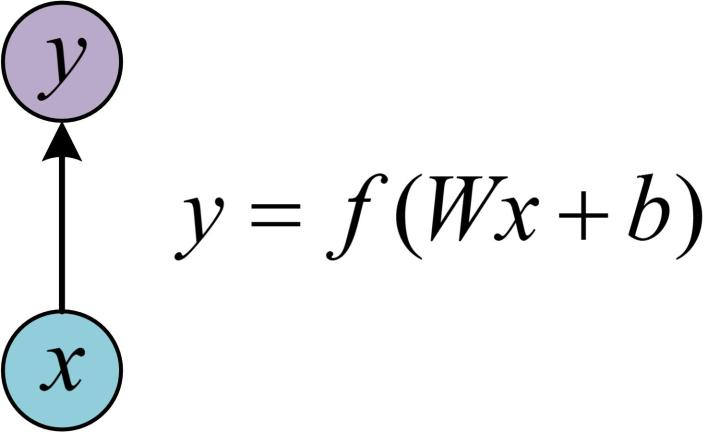
\includegraphics{./img/ch6/6.1.jpg}
%\caption{}
%\end{figure}

\subsection{6.2.2
图解经典RNN结构}\label{ux56feux89e3ux7ecfux5178rnnux7ed3ux6784}

​ 在实际应用中,我们还会遇到很多序列形的数据,如:

\begin{itemize}
\item
  自然语言处理问题。x1可以看做是第一个单词,x2可以看做是第二个单词,依次类推。
\item
  语音处理。此时,x1、x2、x3\ldots{}\ldots{}是每帧的声音信号。
\item
  时间序列问题。例如每天的股票价格等等。
\end{itemize}

其单个序列如下图所示:

%\begin{figure}
%\centering
%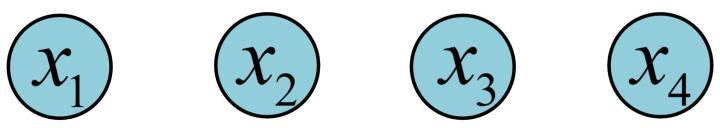
\includegraphics{./img/ch6/6.2.jpg}
%\caption{}
%\end{figure}

前面介绍了诸如此类的序列数据用原始的神经网络难以建模,基于此,RNN引入了隐状态\(h\)(hidden
state),\(h​\)可对序列数据提取特征,接着再转换为输出。

为了便于理解,先计算\(h_1​\):

%\begin{figure}
%\centering
%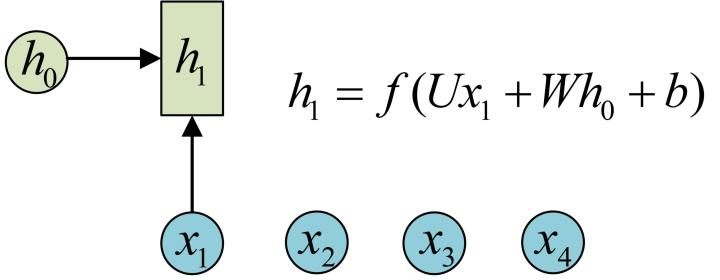
\includegraphics{./img/ch6/6.3.jpg}
%\caption{}
%\end{figure}

注:图中的圆圈表示向量,箭头表示对向量做变换。

RNN中,每个步骤使用的参数\texttt{$U,W,b$}​相同,\texttt{$h\_2$}的计算方式和\texttt{$h\_1​$}类似,其计算结果如下:

%\begin{figure}
%\centering
%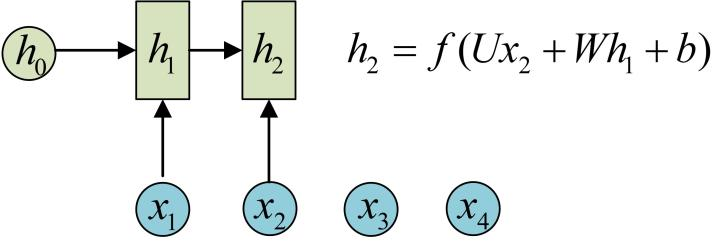
\includegraphics{./img/ch6/6.4.jpg}
%\caption{}
%\end{figure}

计算\(h_3\),\(h_4​\)也相似,可得:

%\begin{figure}
%\centering
%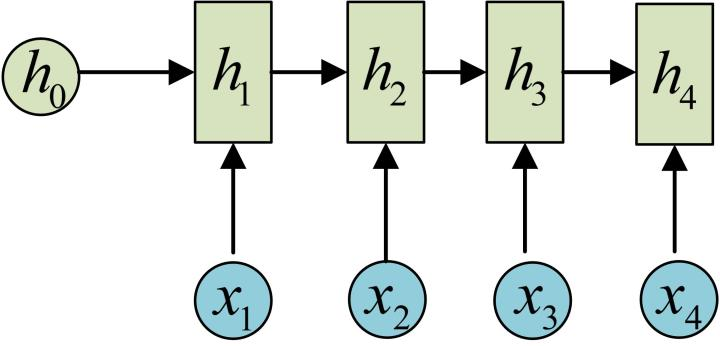
\includegraphics{./img/ch6/6.5.jpg}
%\caption{}
%\end{figure}

接下来,计算RNN的输出\(y_1\),采用\(Softmax\)作为激活函数,根据\(y_n=f(Wx+b)\),得\(y_1​\):

%\begin{figure}
%\centering
%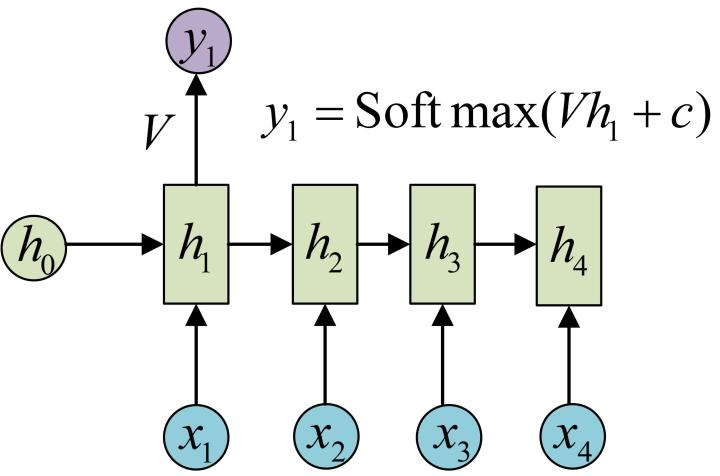
\includegraphics{./img/ch6/6.6.jpg}
%\caption{}
%\end{figure}

使用和\(y_1​\)相同的参数\(V,c​\),得到\(y_1,y_2,y_3,y_4​\)的输出结构:

%\begin{figure}
%\centering
%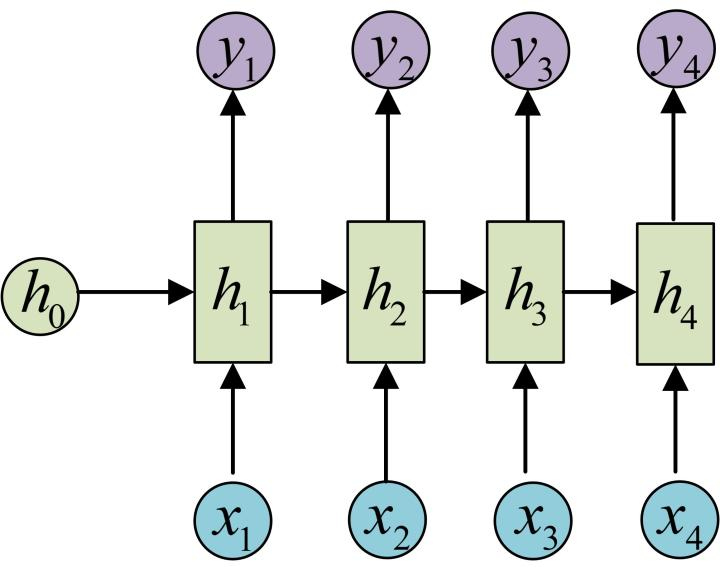
\includegraphics{./img/ch6/6.7.jpg}
%\caption{}
%\end{figure}

以上即为最经典的RNN结构,其输入为\(x_1,x_2,x_3,x_4\),输出为\(y_1,y_2,y_3,y_4\),当然实际中最大值为\(y_n\),这里为了便于理解和展示,只计算4个输入和输出。从以上结构可看出,RNN结构的输入和输出等长。

\subsection{6.2.3
vector-to-sequence结构}\label{vector-to-sequenceux7ed3ux6784}

​
有时我们要处理的问题输入是一个单独的值,输出是一个序列。此时,有两种主要建模方式:

​
方式一:可只在其中的某一个序列进行计算,比如序列第一个进行输入计算,其建模方式如下:

%\begin{figure}
%\centering
%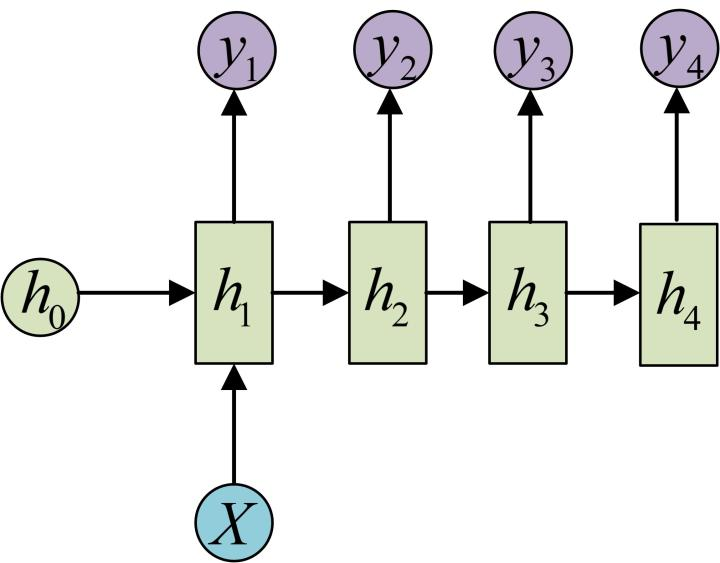
\includegraphics{./img/ch6/6.9.jpg}
%\caption{}
%\end{figure}

​ 方式二:把输入信息X作为每个阶段的输入,其建模方式如下:

%\begin{figure}
%\centering
%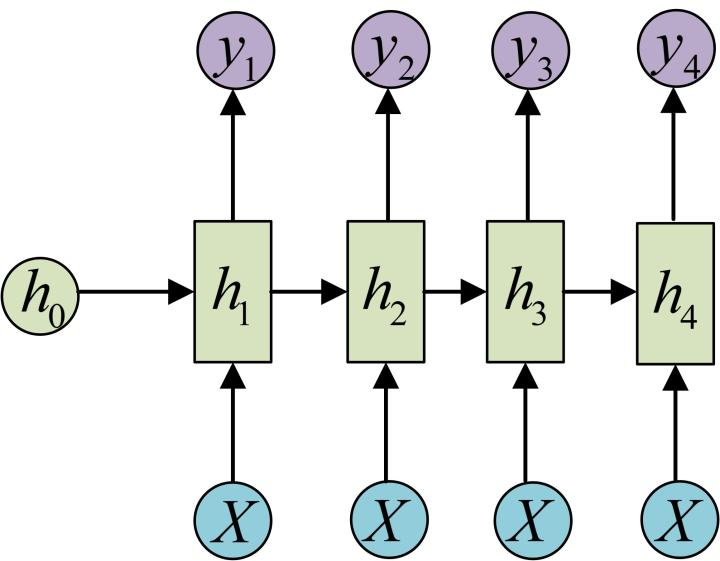
\includegraphics{./img/ch6/6.10.jpg}
%\caption{}
%\end{figure}

\subsection{6.2.4
sequence-to-vector结构}\label{sequence-to-vectorux7ed3ux6784}

​
有时我们要处理的问题输入是一个序列,输出是一个单独的值,此时通常在最后的一个序列上进行输出变换,其建模如下所示:

%\begin{figure}
%\centering
%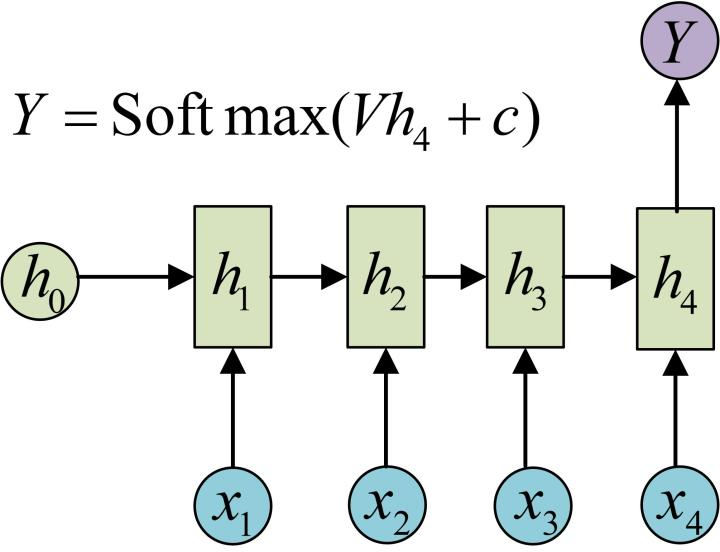
\includegraphics{./img/ch6/6.8.jpg}
%\caption{}
%\end{figure}

\subsection{6.2.5
Encoder-Decoder结构}\label{encoder-decoderux7ed3ux6784}

​
原始的sequence-to-sequence结构的RNN要求序列等长,然而我们遇到的大部分问题序列都是不等长的,如机器翻译中,源语言和目标语言的句子往往并没有相同的长度。

​ 其建模步骤如下:

​
\textbf{步骤一}:将输入数据编码成一个上下文向量\(c\),这部分称为Encoder,得到\(c\)有多种方式,最简单的方法就是把Encoder的最后一个隐状态赋值给\(c\),还可以对最后的隐状态做一个变换得到\(c\),也可以对所有的隐状态做变换。其示意如下所示:

%\begin{figure}
%\centering
%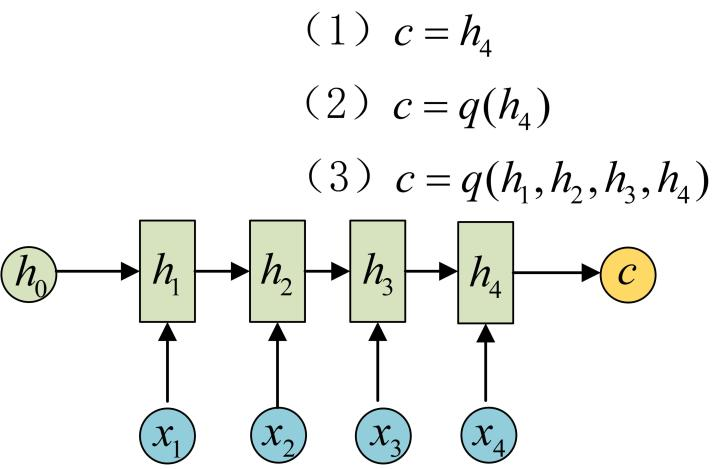
\includegraphics{./img/ch6/6.12.jpg}
%\caption{}
%\end{figure}

​
\textbf{步骤二}:用另一个RNN网络(我们将其称为Decoder)对其进行编码,方法一是将步骤一中的\(c​\)作为初始状态输入到Decoder,示意图如下所示:

%\begin{figure}
%\centering
%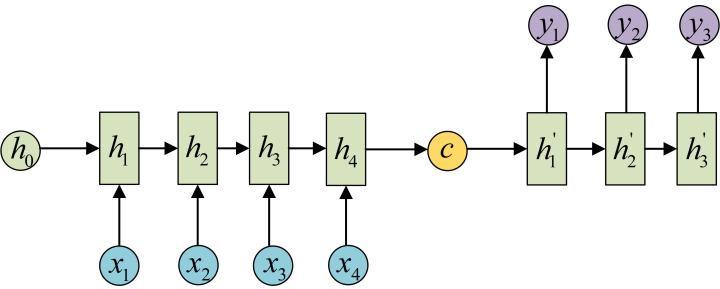
\includegraphics{./img/ch6/6.13.jpg}
%\caption{}
%\end{figure}

方法二是将\(c\)作为Decoder的每一步输入,示意图如下所示:

%\begin{figure}
%\centering
%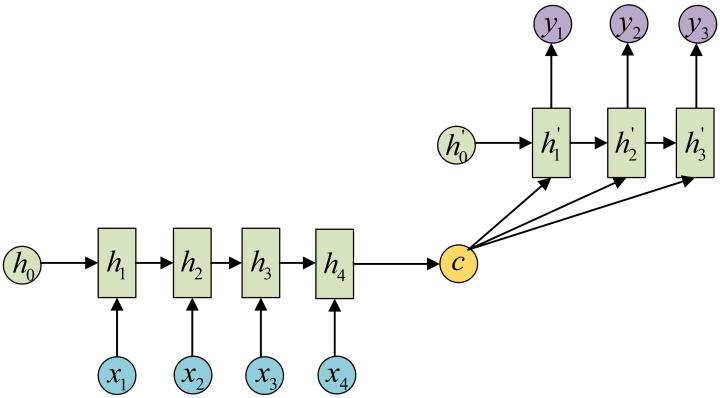
\includegraphics{./img/ch6/6.14.jpg}
%\caption{}
%\end{figure}

\subsection{以上三种结构各有怎样的应用场景}\label{ux4ee5ux4e0aux4e09ux79cdux7ed3ux6784ux5404ux6709ux600eux6837ux7684ux5e94ux7528ux573aux666f}

\begin{longtable}[]{ lcl }
%\toprule
\begin{minipage}[b]{0.09\columnwidth}\raggedright\strut
网络结构\strut
\end{minipage} & \begin{minipage}[b]{0.23\columnwidth}%\centering\strut
结构图示\strut
\end{minipage} & \begin{minipage}[b]{0.59\columnwidth}\raggedright\strut
应用场景举例\strut
\end{minipage}\tabularnewline
%\midrule
%\endhead
\begin{minipage}[t]{0.09\columnwidth}\raggedright\strut
1 vs N\strut
\end{minipage} & \begin{minipage}[t]{0.23\columnwidth}%\centering\strut
%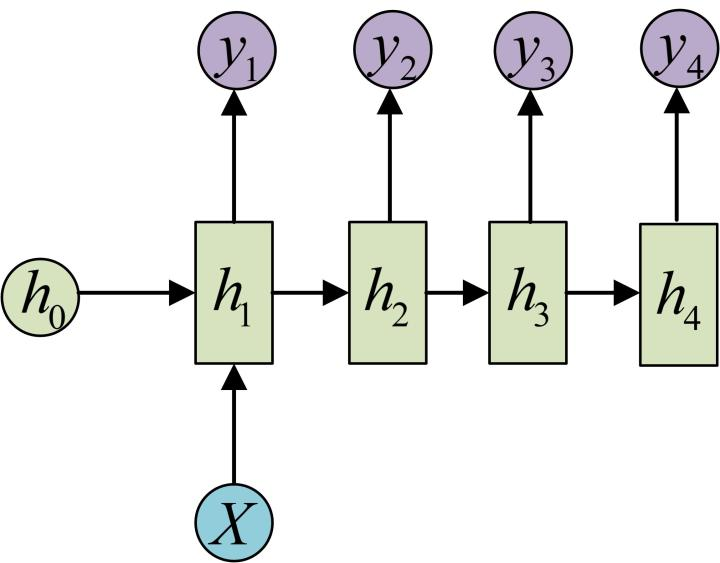
\includegraphics{./img/ch6/6.9.jpg}\strut
\end{minipage} & \begin{minipage}[t]{0.59\columnwidth}\raggedright\strut
1、从图像生成文字,输入为图像的特征,输出为一段句子2、根据图像生成语音或音乐,输入为图像特征,输出为一段语音或音乐\strut
\end{minipage}\tabularnewline
\begin{minipage}[t]{0.09\columnwidth}\raggedright\strut
N vs 1\strut
\end{minipage} & \begin{minipage}[t]{0.23\columnwidth}%\centering\strut
%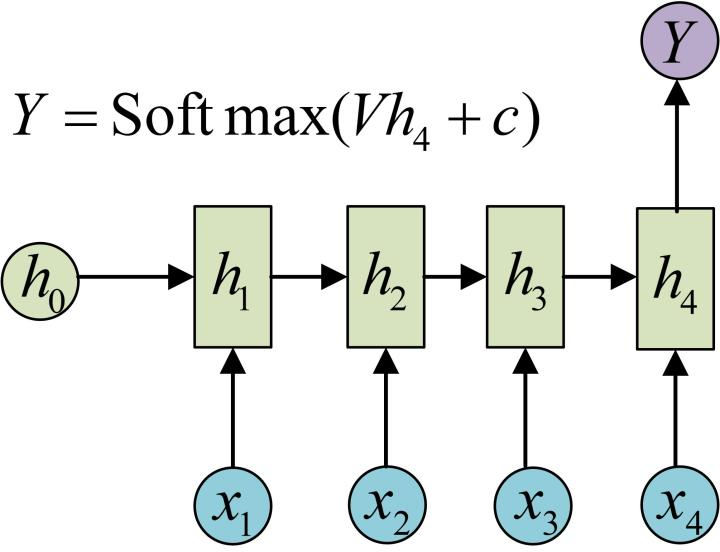
\includegraphics{./img/ch6/6.8.jpg}\strut
\end{minipage} & \begin{minipage}[t]{0.59\columnwidth}\raggedright\strut
1、输出一段文字,判断其所属类别2、输入一个句子,判断其情感倾向3、输入一段视频,判断其所属类别\strut
\end{minipage}\tabularnewline
\begin{minipage}[t]{0.09\columnwidth}\raggedright\strut
N vs M\strut
\end{minipage} & \begin{minipage}[t]{0.23\columnwidth}%\centering\strut
%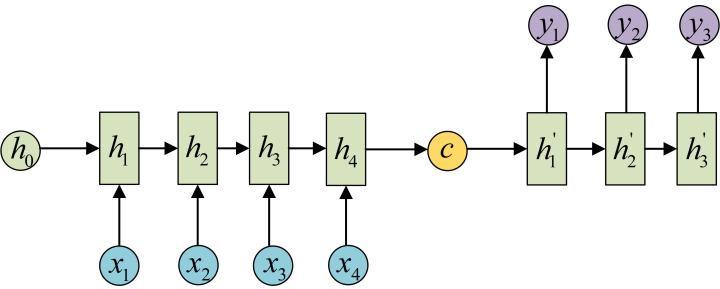
\includegraphics{./img/ch6/6.13.jpg}\strut
\end{minipage} & \begin{minipage}[t]{0.59\columnwidth}\raggedright\strut
1、机器翻译,输入一种语言文本序列,输出另外一种语言的文本序列2、文本摘要,输入文本序列,输出这段文本序列摘要3、阅读理解,输入文章,输出问题答案4、语音识别,输入语音序列信息,输出文字序列\strut
\end{minipage}\tabularnewline
%\bottomrule
\end{longtable}

\subsection{6.2.7
图解RNN中的Attention机制}\label{ux56feux89e3rnnux4e2dux7684attentionux673aux5236}

​
在上述通用的Encoder-Decoder结构中,Encoder把所有的输入序列都编码成一个统一的语义特征\(c​\)再解码,因此,\(c​\)中必须包含原始序列中的所有信息,它的长度就成了限制模型性能的瓶颈。如机器翻译问题,当要翻译的句子较长时,一个\(c​\)可能存不下那么多信息,就会造成翻译精度的下降。Attention机制通过在每个时间输入不同的\(c​\)来解决此问题。

​
引入了Attention机制的Decoder中,有不同的\(c\),每个\(c​\)会自动选择与当前输出最匹配的上下文信息,其示意图如下所示:

%\begin{figure}
%\centering
%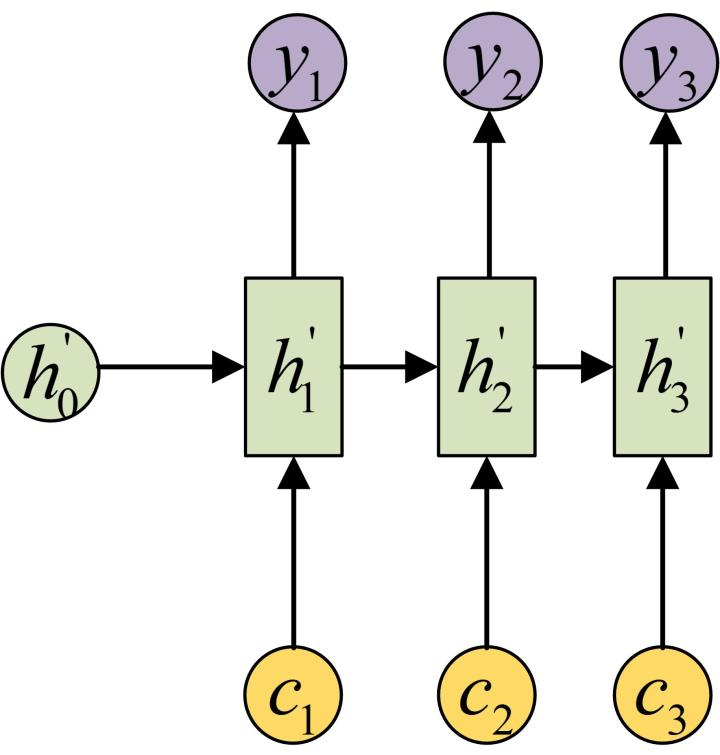
\includegraphics{./img/ch6/6.15.jpg}
%\caption{}
%\end{figure}

​ \textbf{举例},比如输入序列是``我爱中国'',要将此输入翻译成英文:

​
假如用\(a_{ij}\)衡量Encoder中第\(j\)阶段的\(h_j\)和解码时第\(i\)阶段的相关性,\(a_{ij}\)从模型中学习得到,和Decoder的第\(i-1\)阶段的隐状态、Encoder
第\(j\)个阶段的隐状态有关,比如\(a_{3j}​\)的计算示意如下所示:

%\begin{figure}
%\centering
%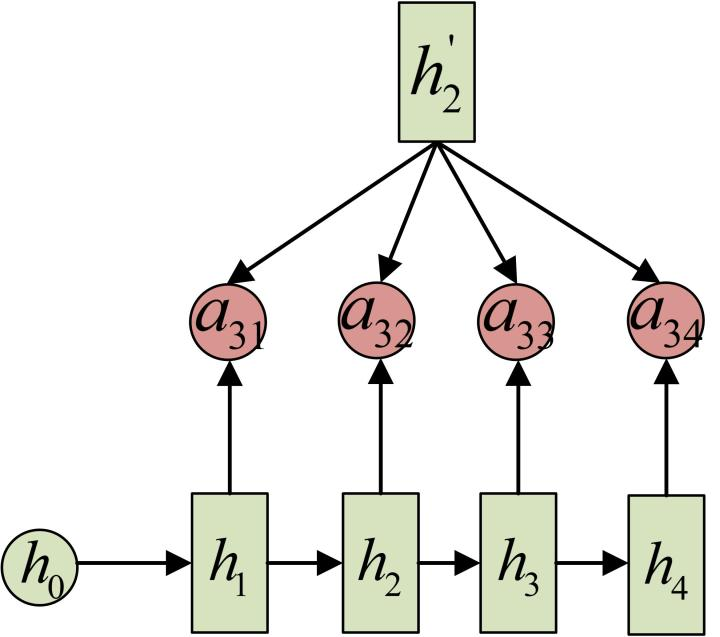
\includegraphics{./img/ch6/6.19.jpg}
%\caption{}
%\end{figure}

最终Decoder中第\(i\)阶段的输入的上下文信息
\(c_i\)来自于所有\(h_j\)对\(a_{ij}\)的加权和。

其示意图如下图所示:

%\begin{figure}
%\centering
%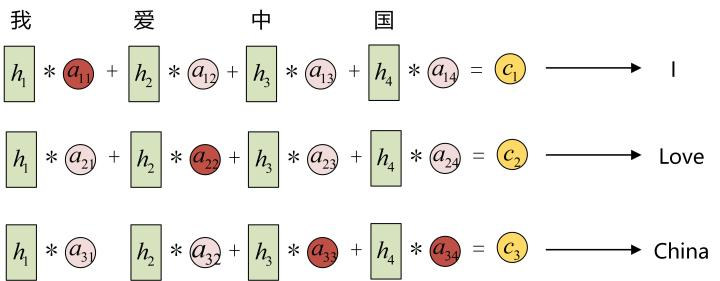
\includegraphics{./img/ch6/6.16.jpg}
%\caption{}
%\end{figure}

​
在Encoder中,\(h_1,h_2,h_3,h_4\)分别代表``我'',``爱'',``中'',``国''所代表信息。翻译的过程中,\(c_1\)会选择和``我''最相关的上下午信息,如上图所示,会优先选择\(a_{11}\),以此类推,\(c_2\)会优先选择相关性较大的\(a_{22}\),\(c_3\)会优先选择相关性较大的\(a_{33},a_{34}\),这就是attention机制。

\section{6.3 RNNs典型特点?}\label{rnnsux5178ux578bux7279ux70b9}

\begin{enumerate}
\def\labelenumi{\arabic{enumi}.}
% \tightlist
\item
  RNNs主要用于处理序列数据。对于传统神经网络模型,从输入层到隐含层再到输出层,层与层之间一般为全连接,每层之间神经元是无连接的。但是传统神经网络无法处理数据间的前后关联问题。例如,为了预测句子的下一个单词,一般需要该词之前的语义信息。这是因为一个句子中前后单词是存在语义联系的。
\item
  RNNs中当前单元的输出与之前步骤输出也有关,因此称之为循环神经网络。具体的表现形式为当前单元会对之前步骤信息进行储存并应用于当前输出的计算中。隐藏层之间的节点连接起来,隐藏层当前输出由当前时刻输入向量和之前时刻隐藏层状态共同决定。
\item
  标准的RNNs结构图,图中每个箭头代表做一次变换,也就是说箭头连接带有权值。
\item
  在标准的RNN结构中,隐层的神经元之间也是带有权值的,且权值共享。
\item
  理论上,RNNs能够对任何长度序列数据进行处理。但是在实践中,为了降低复杂度往往假设当前的状态只与之前某几个时刻状态相关,\textbf{下图便是一个典型的RNNs}:
\end{enumerate}

%\begin{figure}
%\centering
%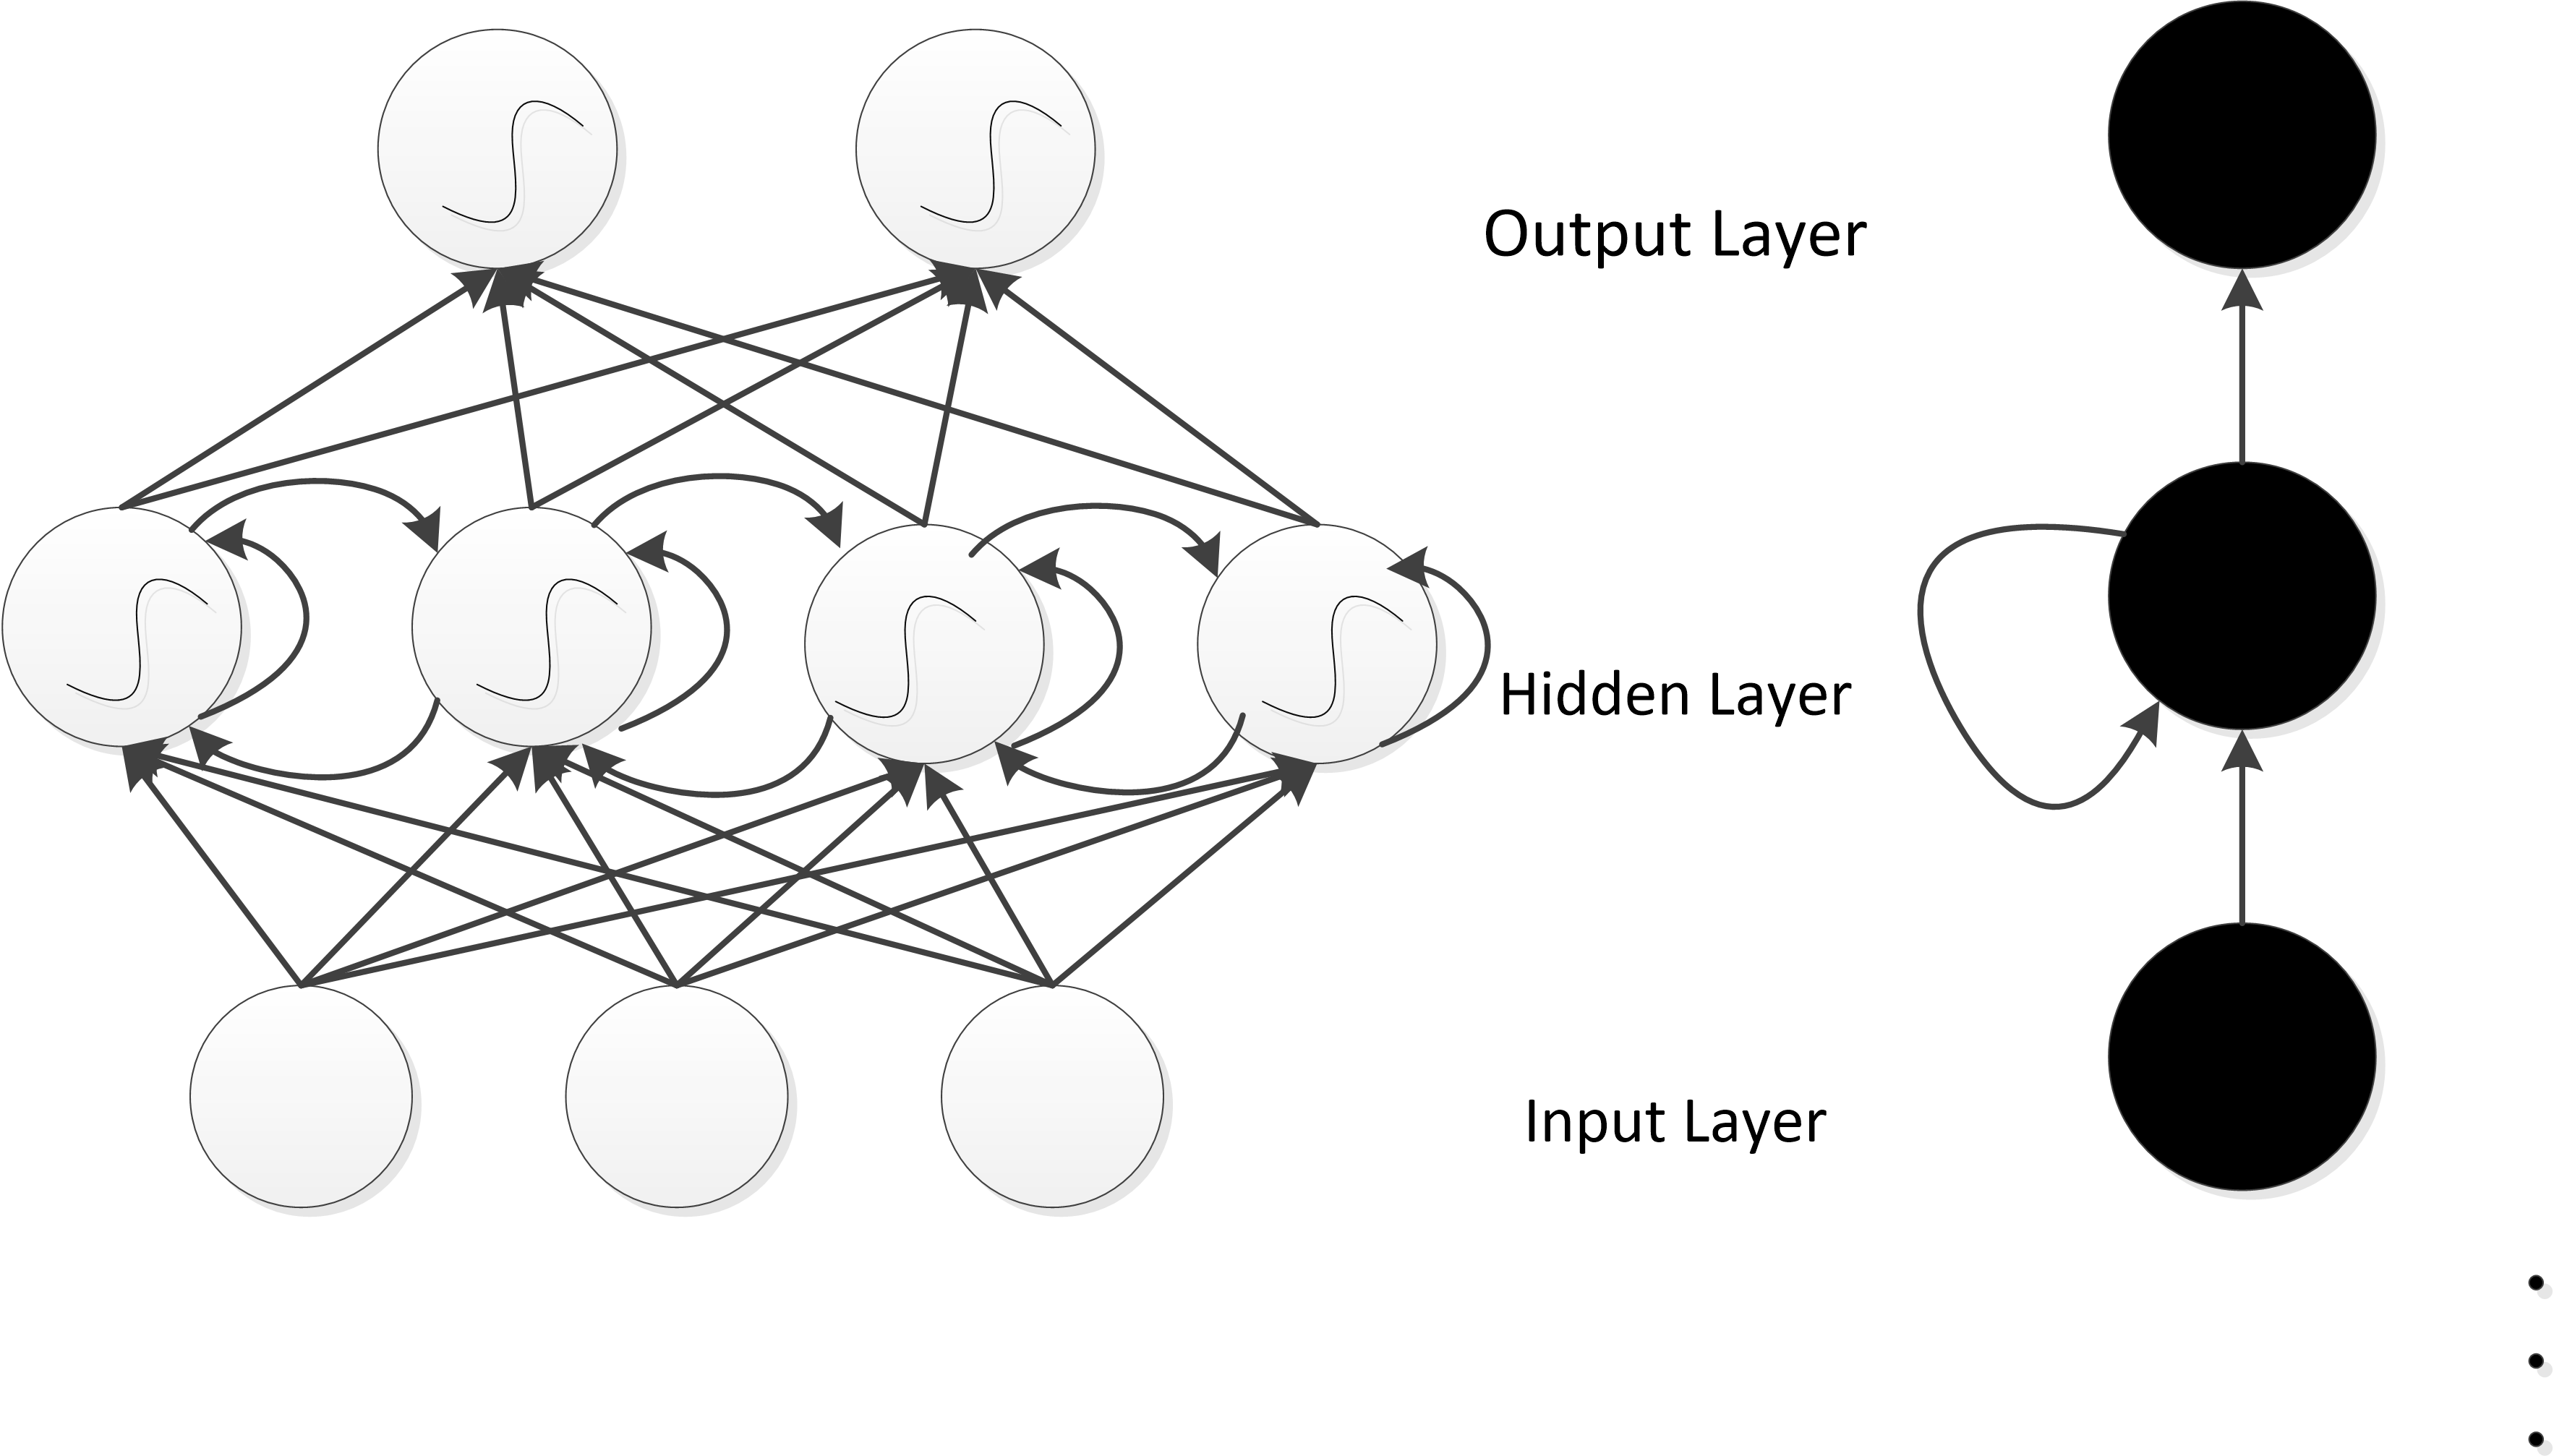
\includegraphics{./img/ch6/figure_6.2_1.png}
%\caption{}
%\end{figure}

%\begin{figure}
%\centering
%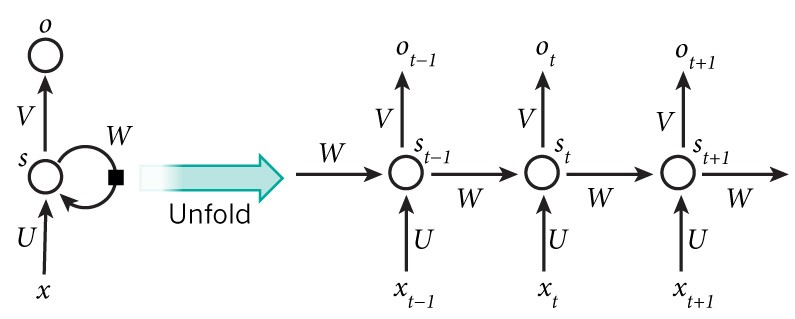
\includegraphics{./img/ch6/figure_6.2_2.jpg}
%\caption{}
%\end{figure}

输入单元(Input
units):输入集\(\bigr\{x_0,x_1,...,x_t,x_{t+1},...\bigr\}\),

输出单元(Output
units):输出集\(\bigr\{y_0,y_1,...,y_t,y_{y+1},...\bigr\}\),

隐藏单元(Hidden
units):输出集\(\bigr\{s_0,s_1,...,s_t,s_{t+1},...\bigr\}\)。

\textbf{图中信息传递特点:}

\begin{enumerate}
\def\labelenumi{\arabic{enumi}.}
% \tightlist
\item
  一条单向流动的信息流是从输入单元到隐藏单元。
\item
  一条单向流动的信息流从隐藏单元到输出单元。
\item
  在某些情况下,RNNs会打破后者的限制,引导信息从输出单元返回隐藏单元,这些被称为``Back
  Projections''。
\item
  在某些情况下,隐藏层的输入还包括上一时刻隐藏层的状态,即隐藏层内的节点可以自连也可以互连。
\item
  当前单元(cell)输出是由当前时刻输入和上一时刻隐藏层状态共同决定。
\end{enumerate}

\section{6.4 CNN和RNN的区别 ?}\label{cnnux548crnnux7684ux533aux522b}

\begin{longtable}[]{ ll }
%\toprule
\begin{minipage}[b]{0.09\columnwidth}\raggedright\strut
类别\strut
\end{minipage} & \begin{minipage}[b]{0.80\columnwidth}\raggedright\strut
特点描述\strut
\end{minipage}\tabularnewline
%\midrule
%\endhead
\begin{minipage}[t]{0.09\columnwidth}\raggedright\strut
相同点\strut
\end{minipage} & \begin{minipage}[t]{0.80\columnwidth}\raggedright\strut
1、传统神经网络的扩展。2、前向计算产生结果,反向计算模型更新。3、每层神经网络横向可以多个神经元共存,纵向可以有多层神经网络连接。\strut
\end{minipage}\tabularnewline
\begin{minipage}[t]{0.09\columnwidth}\raggedright\strut
不同点\strut
\end{minipage} & \begin{minipage}[t]{0.80\columnwidth}\raggedright\strut
1、CNN空间扩展,神经元与特征卷积;RNN时间扩展,神经元与多个时间输出计算2、RNN可以用于描述时间上连续状态的输出,有记忆功能,CNN用于静态输出\strut
\end{minipage}\tabularnewline
%\bottomrule
\end{longtable}

\section{6.5
RNNs和FNNs有什么区别?}\label{rnnsux548cfnnsux6709ux4ec0ux4e48ux533aux522b}

\begin{enumerate}
\def\labelenumi{\arabic{enumi}.}
% \tightlist
\item
  不同于传统的前馈神经网络(FNNs),RNNs引入了定向循环,能够处理输入之间前后关联问题。
\item
  RNNs可以记忆之前步骤的训练信息。 \textbf{定向循环结构如下图所示}:
\end{enumerate}

%\begin{figure}
%\centering
%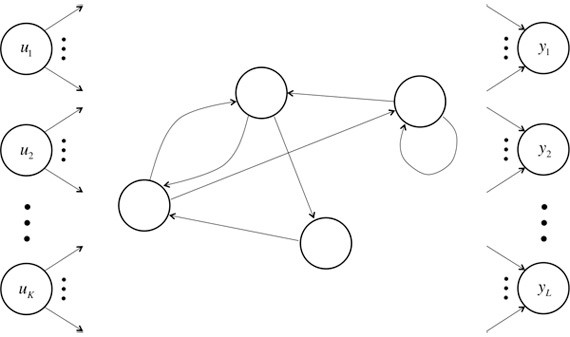
\includegraphics{./img/ch6/figure_6.1_1.jpg}
%\caption{}
%\end{figure}

\section{6.6
RNNs训练和传统ANN训练异同点?}\label{rnnsux8badux7ec3ux548cux4f20ux7edfannux8badux7ec3ux5f02ux540cux70b9}

\textbf{相同点}:

\begin{enumerate}
\def\labelenumi{\arabic{enumi}.}
% \tightlist
\item
  RNNs与传统ANN都使用BP(Back Propagation)误差反向传播算法。
\end{enumerate}

\textbf{不同点}:

\begin{enumerate}
\def\labelenumi{\arabic{enumi}.}
% \tightlist
\item
  RNNs网络参数W,U,V是共享的(具体在本章6.2节中已介绍),而传统神经网络各层参数间没有直接联系。
\item
  对于RNNs,在使用梯度下降算法中,每一步的输出不仅依赖当前步的网络,还依赖于之前若干步的网络状态。
\end{enumerate}

\section{6.7 为什么RNN
训练的时候Loss波动很大}\label{ux4e3aux4ec0ux4e48rnn-ux8badux7ec3ux7684ux65f6ux5019lossux6ce2ux52a8ux5f88ux5927}

​ 由于RNN特有的memory会影响后期其他的RNN的特点,梯度时大时小,learning
rate没法个性化的调整,导致RNN在train的过程中,Loss会震荡起伏,为了解决RNN的这个问题,在训练的时候,可以设置临界值,当梯度大于某个临界值,直接截断,用这个临界值作为梯度的大小,防止大幅震荡。

\section{6.8
标准RNN前向输出流程}\label{ux6807ux51c6rnnux524dux5411ux8f93ux51faux6d41ux7a0b}

​
以\(x\)表示输入,\(h\)是隐层单元,\(o\)是输出,\(L\)为损失函数,\(y\)为训练集标签。\(t\)表示\(t\)时刻的状态,\(V,U,W\)是权值,同一类型的连接权值相同。以下图为例进行说明标准RNN的前向传播算法:

​ %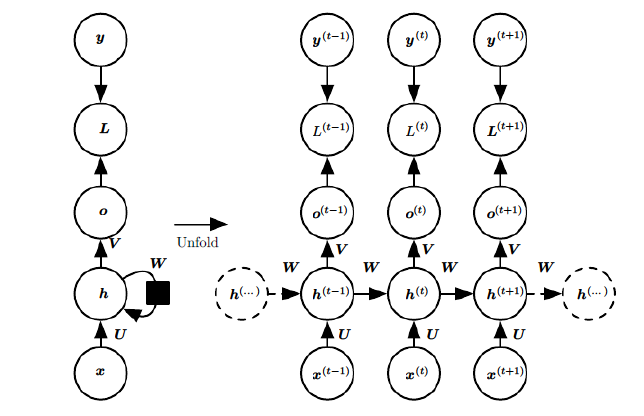
\includegraphics{./img/ch6/rnnbp.png}

对于\(t\)时刻: \[
h^{(t)}=\phi(Ux^{(t)}+Wh^{(t-1)}+b)
\] 其中\(\phi()\)为激活函数,一般会选择tanh函数,\(b\)为偏置。

\(t\)时刻的输出为: \[
o^{(t)}=Vh^{(t)}+c
\] 模型的预测输出为: \[
\widehat{y}^{(t)}=\sigma(o^{(t)})
\] 其中\(\sigma​\)为激活函数,通常RNN用于分类,故这里一般用softmax函数。

\section{6.9 BPTT算法推导}\label{bpttux7b97ux6cd5ux63a8ux5bfc}

​ BPTT(back-propagation through
time)算法是常用的训练RNN的方法,其本质还是BP算法,只不过RNN处理时间序列数据,所以要基于时间反向传播,故叫随时间反向传播。BPTT的中心思想和BP算法相同,沿着需要优化的参数的负梯度方向不断寻找更优的点直至收敛。需要寻优的参数有三个,分别是U、V、W。与BP算法不同的是,其中W和U两个参数的寻优过程需要追溯之前的历史数据,参数V相对简单只需关注目前,那么我们就来先求解参数V的偏导数。
\[
\frac{\partial L^{(t)}}{\partial V}=\frac{\partial L^{(t)}}{\partial o^{(t)}}\cdot \frac{\partial o^{(t)}}{\partial V}
\] RNN的损失也是会随着时间累加的,所以不能只求t时刻的偏导。 \[
L=\sum_{t=1}^{n}L^{(t)}
\]

\[
\frac{\partial L}{\partial V}=\sum_{t=1}^{n}\frac{\partial L^{(t)}}{\partial o^{(t)}}\cdot \frac{\partial o^{(t)}}{\partial V}
\]

​
W和U的偏导的求解由于需要涉及到历史数据,其偏导求起来相对复杂。为了简化推导过程,我们假设只有三个时刻,那么在第三个时刻
L对W,L对U的偏导数分别为: \[
\frac{\partial L^{(3)}}{\partial W}=\frac{\partial L^{(3)}}{\partial o^{(3)}}\frac{\partial o^{(3)}}{\partial h^{(3)}}\frac{\partial h^{(3)}}{\partial W}+\frac{\partial L^{(3)}}{\partial o^{(3)}}\frac{\partial o^{(3)}}{\partial h^{(3)}}\frac{\partial h^{(3)}}{\partial h^{(2)}}\frac{\partial h^{(2)}}{\partial W}+\frac{\partial L^{(3)}}{\partial o^{(3)}}\frac{\partial o^{(3)}}{\partial h^{(3)}}\frac{\partial h^{(3)}}{\partial h^{(2)}}\frac{\partial h^{(2)}}{\partial h^{(1)}}\frac{\partial h^{(1)}}{\partial W}
\]

\[
\frac{\partial L^{(3)}}{\partial U}=\frac{\partial L^{(3)}}{\partial o^{(3)}}\frac{\partial o^{(3)}}{\partial h^{(3)}}\frac{\partial h^{(3)}}{\partial U}+\frac{\partial L^{(3)}}{\partial o^{(3)}}\frac{\partial o^{(3)}}{\partial h^{(3)}}\frac{\partial h^{(3)}}{\partial h^{(2)}}\frac{\partial h^{(2)}}{\partial U}+\frac{\partial L^{(3)}}{\partial o^{(3)}}\frac{\partial o^{(3)}}{\partial h^{(3)}}\frac{\partial h^{(3)}}{\partial h^{(2)}}\frac{\partial h^{(2)}}{\partial h^{(1)}}\frac{\partial h^{(1)}}{\partial U}
\]

可以观察到,在某个时刻的对W或是U的偏导数,需要追溯这个时刻之前所有时刻的信息。根据上面两个式子得出L在t时刻对W和U偏导数的通式:
\[
\frac{\partial L^{(t)}}{\partial W}=\sum_{k=0}^{t}\frac{\partial L^{(t)}}{\partial o^{(t)}}\frac{\partial o^{(t)}}{\partial h^{(t)}}(\prod_{j=k+1}^{t}\frac{\partial h^{(j)}}{\partial h^{(j-1)}})\frac{\partial h^{(k)}}{\partial W}
\]

\[
\frac{\partial L^{(t)}}{\partial U}=\sum_{k=0}^{t}\frac{\partial L^{(t)}}{\partial o^{(t)}}\frac{\partial o^{(t)}}{\partial h^{(t)}}(\prod_{j=k+1}^{t}\frac{\partial h^{(j)}}{\partial h^{(j-1)}})\frac{\partial h^{(k)}}{\partial U}
\]

整体的偏导公式就是将其按时刻再一一加起来。

\section{6.9
RNN中为什么会出现梯度消失?}\label{rnnux4e2dux4e3aux4ec0ux4e48ux4f1aux51faux73b0ux68afux5ea6ux6d88ux5931}

首先来看tanh函数的函数及导数图如下所示:

%\begin{figure}
%\centering
%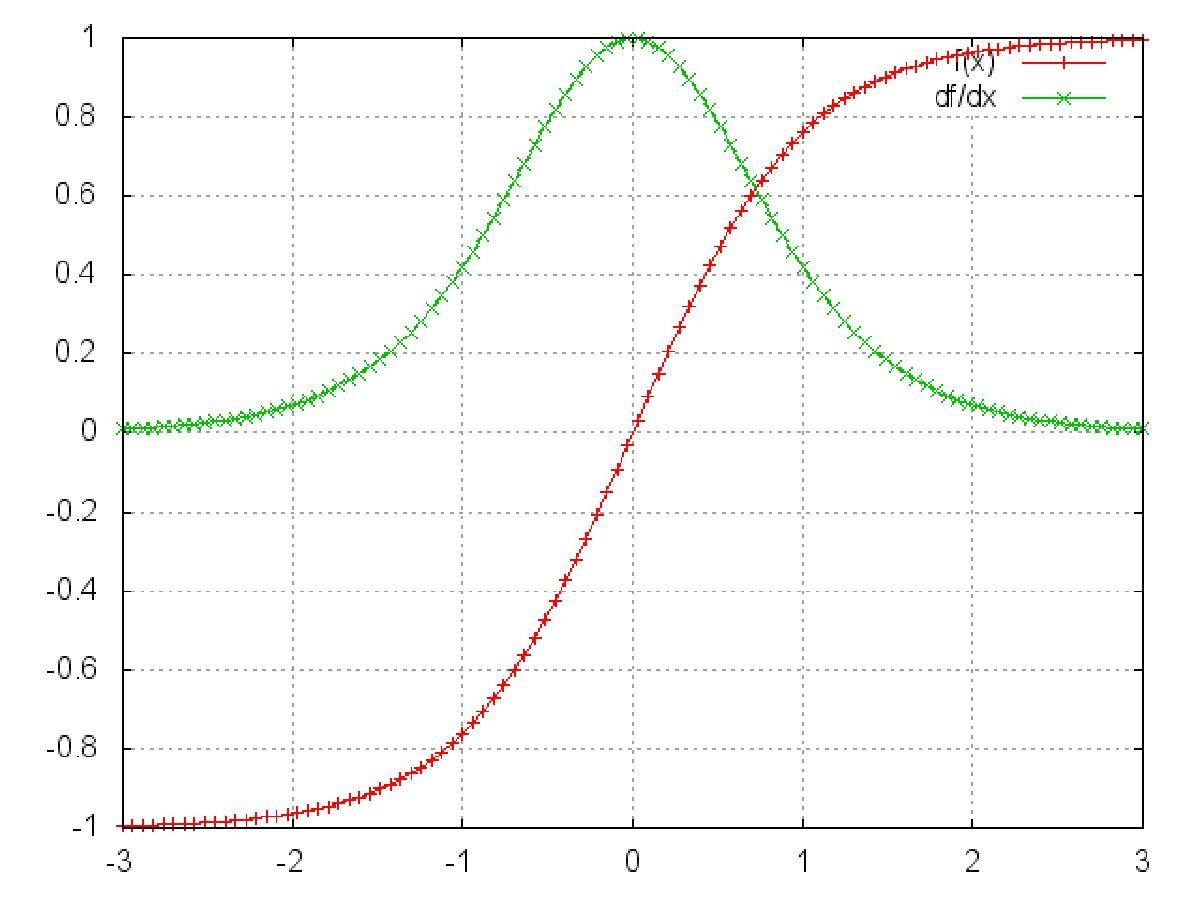
\includegraphics{./img/ch6/tanh.jpg}
%\caption{}
%\end{figure}

sigmoid函数的函数及导数图如下所示:

%\begin{figure}
%\centering
%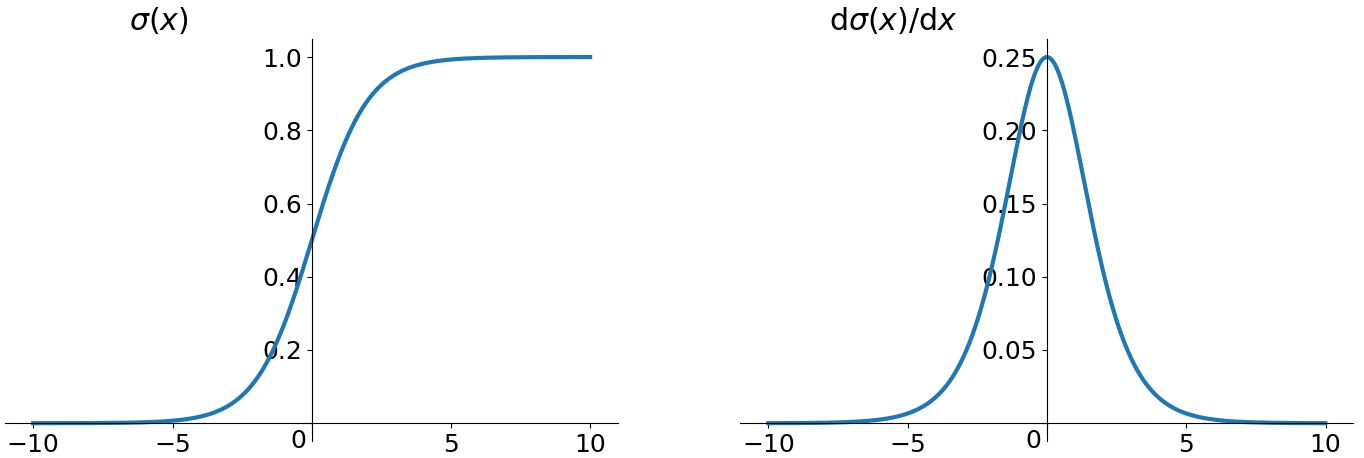
\includegraphics{./img/ch6/sigmoid.jpg}
%\caption{}
%\end{figure}

从上图观察可知,sigmoid函数的导数范围是(0,0.25{]},tanh函数的导数范围是(0,1{]},他们的导数最大都不大于1。

​
基于6.8中式(9-10)中的推导,RNN的激活函数是嵌套在里面的,如果选择激活函数为\(tanh\)或\(sigmoid\),把激活函数放进去,拿出中间累乘的那部分可得:
\[
\prod_{j=k+1}^{t}{\frac{\partial{h^{j}}}{\partial{h^{j-1}}}} = \prod_{j=k+1}^{t}{tanh^{'}}\cdot W_{s}
\]

\[
\prod_{j=k+1}^{t}{\frac{\partial{h^{j}}}{\partial{h^{j-1}}}} = \prod_{j=k+1}^{t}{sigmoid^{'}}\cdot W_{s}
\]

​
\textbf{梯度消失现象}:基于上式,会发现累乘会导致激活函数导数的累乘,如果取tanh或sigmoid函数作为激活函数的话,那么必然是一堆小数在做乘法,结果就是越乘越小。随着时间序列的不断深入,小数的累乘就会导致梯度越来越小直到接近于0,这就是``梯度消失``现象。

​
实际使用中,会优先选择tanh函数,原因是tanh函数相对于sigmoid函数来说梯度较大,收敛速度更快且引起梯度消失更慢。

\section{6.10
如何解决RNN中的梯度消失问题?}\label{ux5982ux4f55ux89e3ux51b3rnnux4e2dux7684ux68afux5ea6ux6d88ux5931ux95eeux9898}

​
上节描述的梯度消失是在无限的利用历史数据而造成,但是RNN的特点本来就是能利用历史数据获取更多的可利用信息,解决RNN中的梯度消失方法主要有:

​
1、选取更好的激活函数,如Relu激活函数。ReLU函数的左侧导数为0,右侧导数恒为1,这就避免了``梯度消失``的发生。但恒为1的导数容易导致``梯度爆炸``,但设定合适的阈值可以解决这个问题。

​
2、加入BN层,其优点包括可加速收敛、控制过拟合,可以少用或不用Dropout和正则、降低网络对初始化权重不敏感,且能允许使用较大的学习率等。

​
2、改变传播结构,LSTM结构可以有效解决这个问题。下面将介绍LSTM相关内容。

\section{6.11 LSTM}\label{lstm}

\subsection{6.11.1
LSTM的产生原因}\label{lstmux7684ux4ea7ux751fux539fux56e0}

​
RNN在处理长期依赖(时间序列上距离较远的节点)时会遇到巨大的困难,因为计算距离较远的节点之间的联系时会涉及雅可比矩阵的多次相乘,会造成梯度消失或者梯度膨胀的现象。为了解决该问题,研究人员提出了许多解决办法,例如ESN(Echo
State Network),增加有漏单元(Leaky
Units)等等。其中最成功应用最广泛的就是门限RNN(Gated
RNN),而LSTM就是门限RNN中最著名的一种。有漏单元通过设计连接间的权重系数,从而允许RNN累积距离较远节点间的长期联系;而门限RNN则泛化了这样的思想,允许在不同时刻改变该系数,且允许网络忘记当前已经累积的信息。

\subsection{6.11.2
图解标准RNN和LSTM的区别}\label{ux56feux89e3ux6807ux51c6rnnux548clstmux7684ux533aux522b}

​ 所有 RNN 都具有一种重复神经网络模块的链式的形式。在标准的 RNN
中,这个重复的模块只有一个非常简单的结构,例如一个 tanh 层,如下图所示:

%\begin{figure}
%\centering
%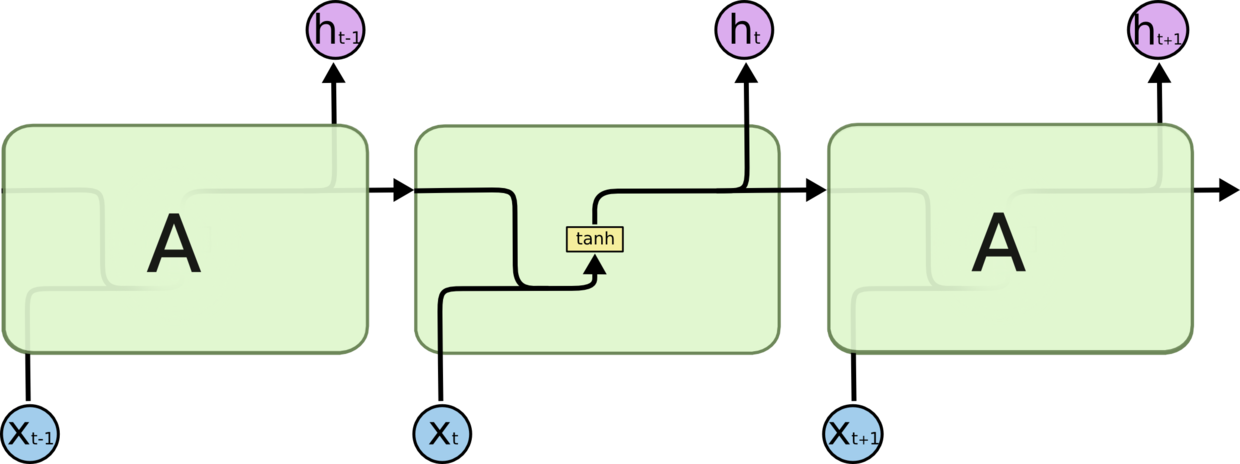
\includegraphics{./img/ch6/LSTM1.png}
%\caption{}
%\end{figure}

​ LSTM
同样是这样的结构,但是重复的模块拥有一个不同的结构。不同于单一神经网络层,这里是有四个,以一种非常特殊的方式进行交互。

%\begin{figure}
%\centering
%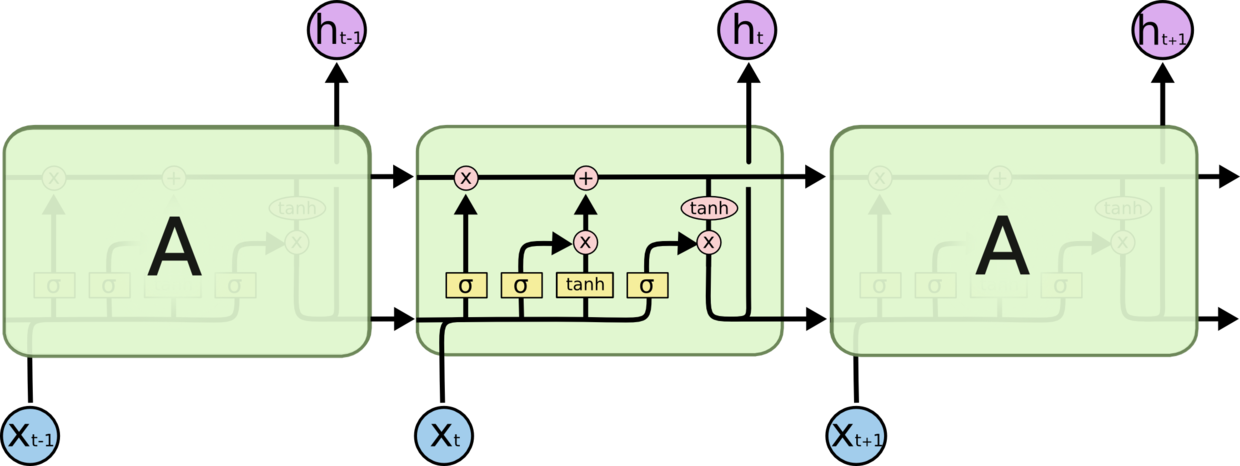
\includegraphics{./img/ch6/LSTM2.png}
%\caption{}
%\end{figure}

注:上图图标具体含义如下所示:

%\begin{figure}
%\centering
%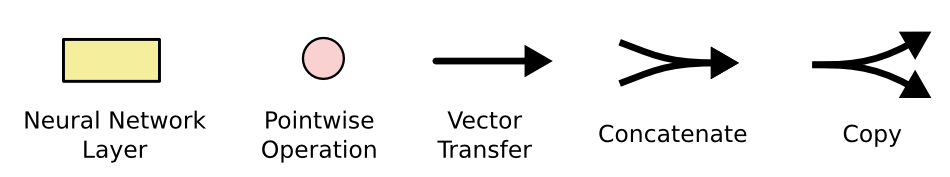
\includegraphics{./img/ch6/LSTM3.png}
%\caption{}
%\end{figure}

​
上图中,每一条黑线传输着一整个向量,从一个节点的输出到其他节点的输入。粉色的圈代表
pointwise
的操作,诸如向量的和,而黄色的矩阵就是学习到的神经网络层。合在一起的线表示向量的连接,分开的线表示内容被复制,然后分发到不同的位置。

\subsection{6.11.3
LSTM核心思想图解}\label{lstmux6838ux5fc3ux601dux60f3ux56feux89e3}

​ LSTM
的关键就是细胞状态,水平线在图上方贯穿运行。细胞状态类似于传送带。直接在整个链上运行,只有一些少量的线性交互。信息在上面流传保持不变会很容易。示意图如下所示:

%\begin{figure}
%\centering
%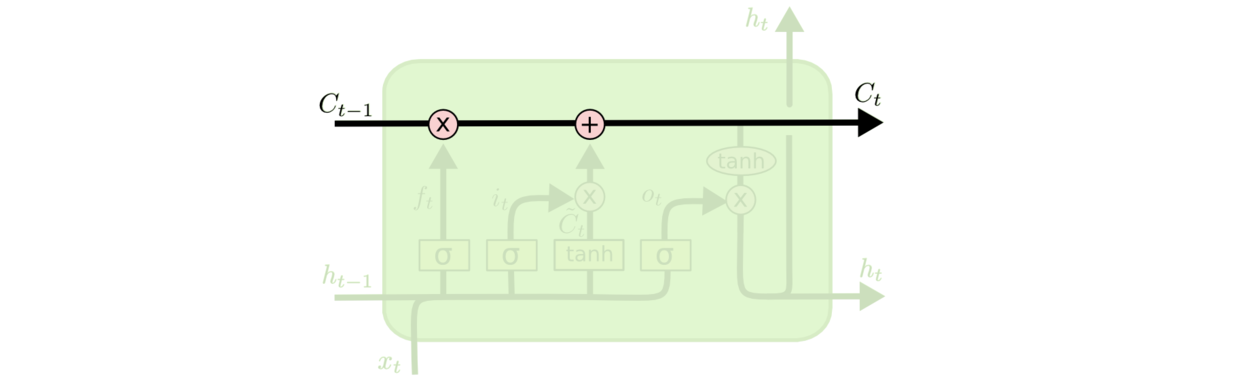
\includegraphics{./img/ch6/LSTM4.png}
%\caption{}
%\end{figure}

LSTM
有通过精心设计的称作为``门''的结构来去除或者增加信息到细胞状态的能力。门是一种让信息选择式通过的方法。他们包含一个
sigmoid 神经网络层和一个 pointwise 乘法操作。示意图如下:

%\begin{figure}
%\centering
%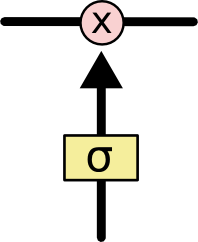
\includegraphics{./img/ch6/LSTM5.png}
%\caption{}
%\end{figure}

LSTM
拥有三个门,分别是忘记层门,输入层门和输出层门,来保护和控制细胞状态。

\textbf{忘记层门}

​ 作用对象:细胞状态 。

​ 作用:将细胞状态中的信息选择性的遗忘。

​ 操作步骤:该门会读取\(h_{t-1}\)和\(x_t\),输出一个在 0 到 1
之间的数值给每个在细胞状态\(C_{t-1}​\)中的数字。1 表示``完全保留'',0
表示``完全舍弃''。示意图如下:

%\begin{figure}
%\centering
%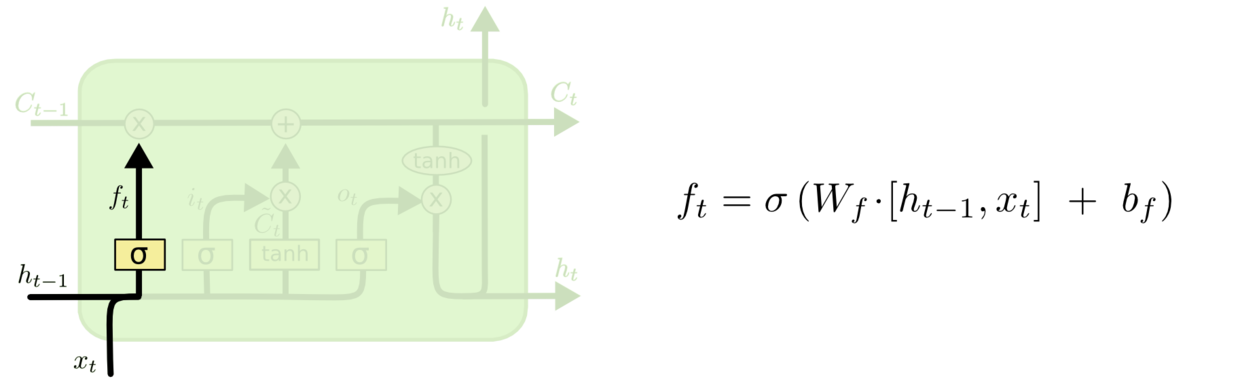
\includegraphics{./img/ch6/LSTM6.png}
%\caption{}
%\end{figure}

\textbf{输入层门}

​ 作用对象:细胞状态

​ 作用:将新的信息选择性的记录到细胞状态中。

​ 操作步骤:

​ 步骤一,sigmoid 层称 ``输入门层'' 决定什么值我们将要更新。

​ 步骤二,tanh
层创建一个新的候选值向量\(\tilde{C}_t\)加入到状态中。其示意图如下:

%\begin{figure}
%\centering
%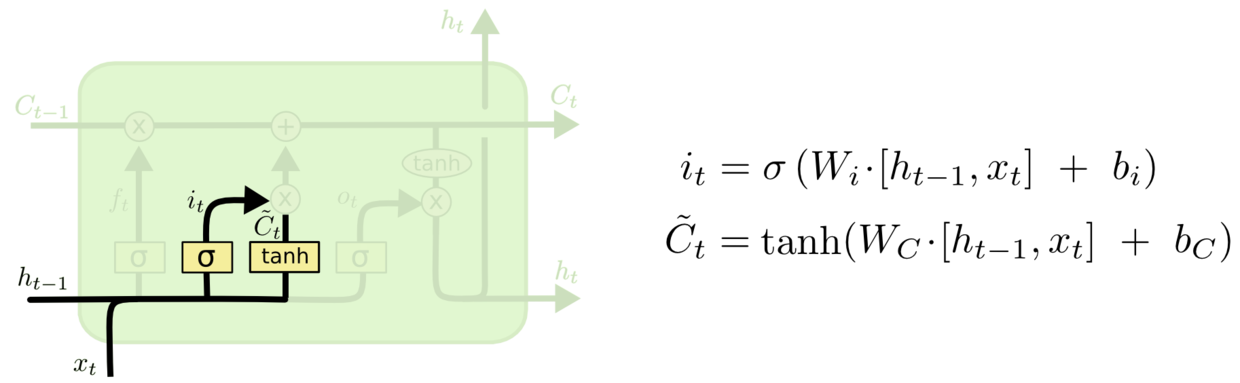
\includegraphics{./img/ch6/LSTM7.png}
%\caption{}
%\end{figure}

​
步骤三:将\(c_{t-1}\)更新为\(c_{t}\)。将旧状态与\(f_t\)相乘,丢弃掉我们确定需要丢弃的信息。接着加上\(i_t * \tilde{C}_t\)得到新的候选值,根据我们决定更新每个状态的程度进行变化。其示意图如下:

%\begin{figure}
%\centering
%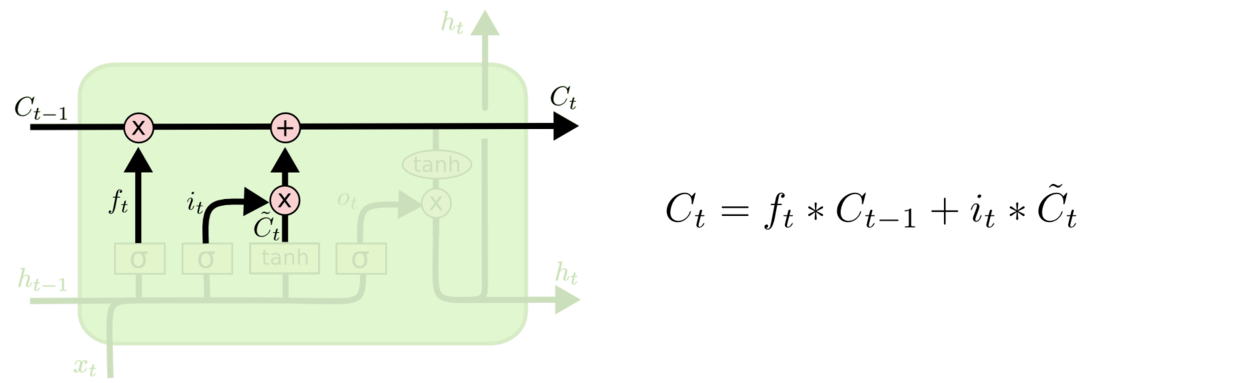
\includegraphics{./img/ch6/LSTM8.png}
%\caption{}
%\end{figure}

\textbf{输出层门} 作用对象:隐层\(h_t\)

​ 作用:确定输出什么值。

​ 操作步骤:

​ 步骤一:通过sigmoid 层来确定细胞状态的哪个部分将输出。

​ 步骤二:把细胞状态通过 tanh 进行处理,并将它和 sigmoid
门的输出相乘,最终我们仅仅会输出我们确定输出的那部分。

其示意图如下所示:

%\begin{figure}
%\centering
%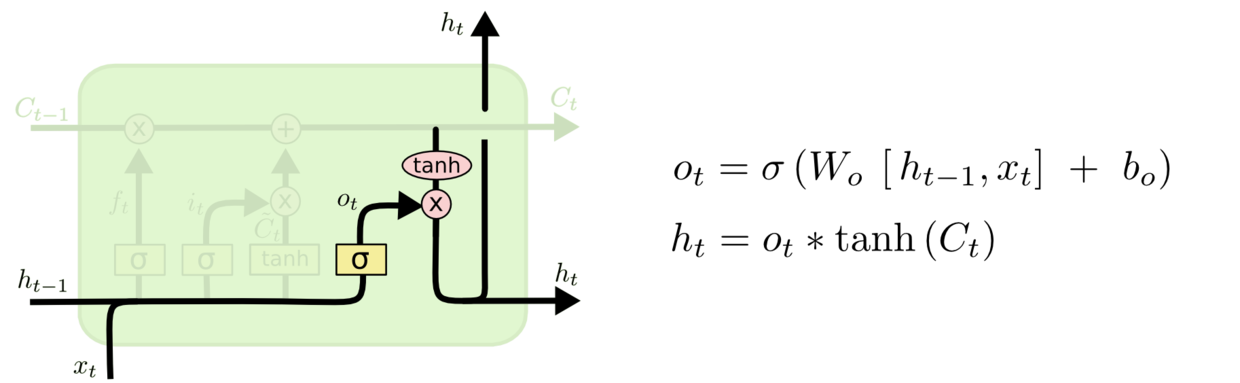
\includegraphics{./img/ch6/LSTM9.png}
%\caption{}
%\end{figure}

\subsection{6.11.4
LSTM流行的变体}\label{lstmux6d41ux884cux7684ux53d8ux4f53}

\textbf{增加peephole 连接}

​ 在正常的LSTM结构中,Gers F A 等人提出增加peephole
连接,可以门层接受细胞状态的输入。示意图如下所示:

%\begin{figure}
%\centering
%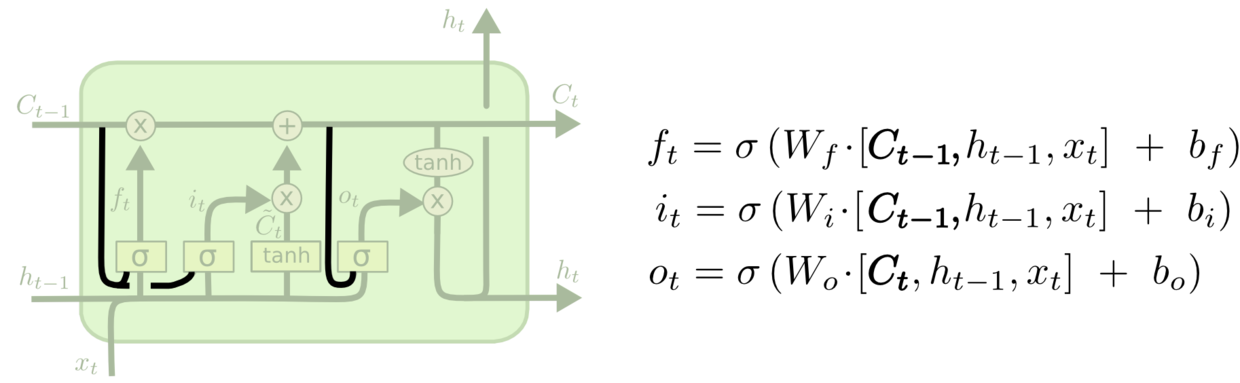
\includegraphics{./img/ch6/LSTM10.png}
%\caption{}
%\end{figure}

\textbf{对忘记门和输入门进行同时确定}

​
不同于之前是分开确定什么忘记和需要添加什么新的信息,这里是一同做出决定。示意图如下所示:

%\begin{figure}
%\centering
%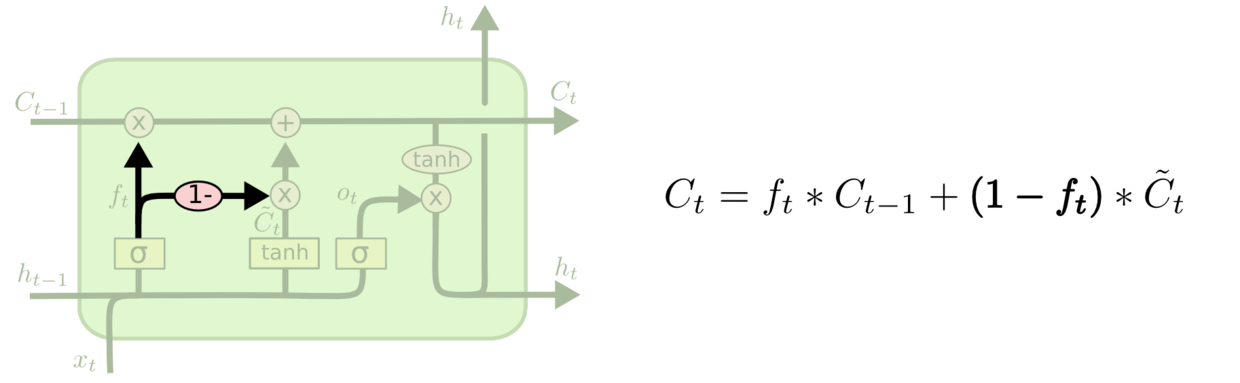
\includegraphics{./img/ch6/LSTM11.png}
%\caption{}
%\end{figure}

\textbf{Gated Recurrent Unit}

​ 由Kyunghyun Cho等人提出的Gated Recurrent Unit
(GRU),其将忘记门和输入门合成了一个单一的更新门,同样还混合了细胞状态和隐藏状态,和其他一些改动。其示意图如下:

%\begin{figure}
%\centering
%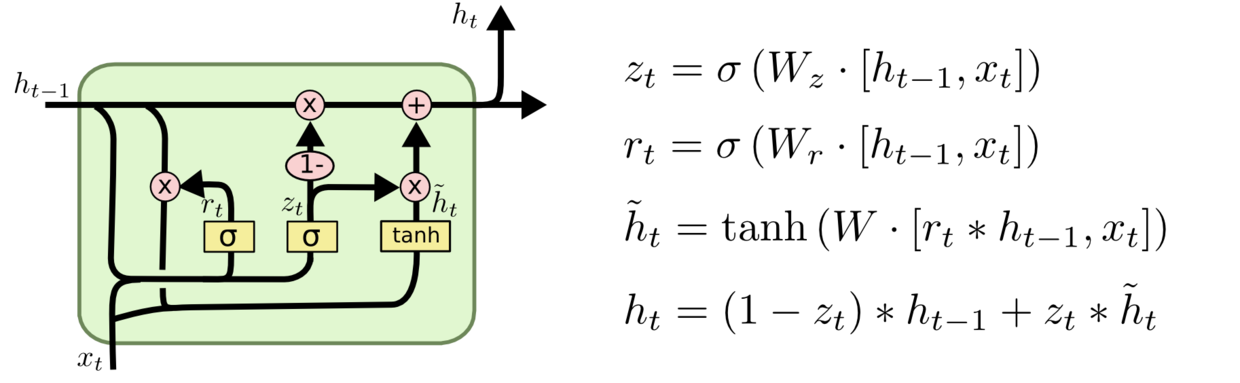
\includegraphics{./img/ch6/LSTM12.png}
%\caption{}
%\end{figure}

最终的模型比标准的 LSTM 模型要简单,也是非常流行的变体。

\section{6.12
LSTMs与GRUs的区别}\label{lstmsux4e0egrusux7684ux533aux522b}

LSTMs与GRUs的区别如图所示:

%\begin{figure}
%\centering
%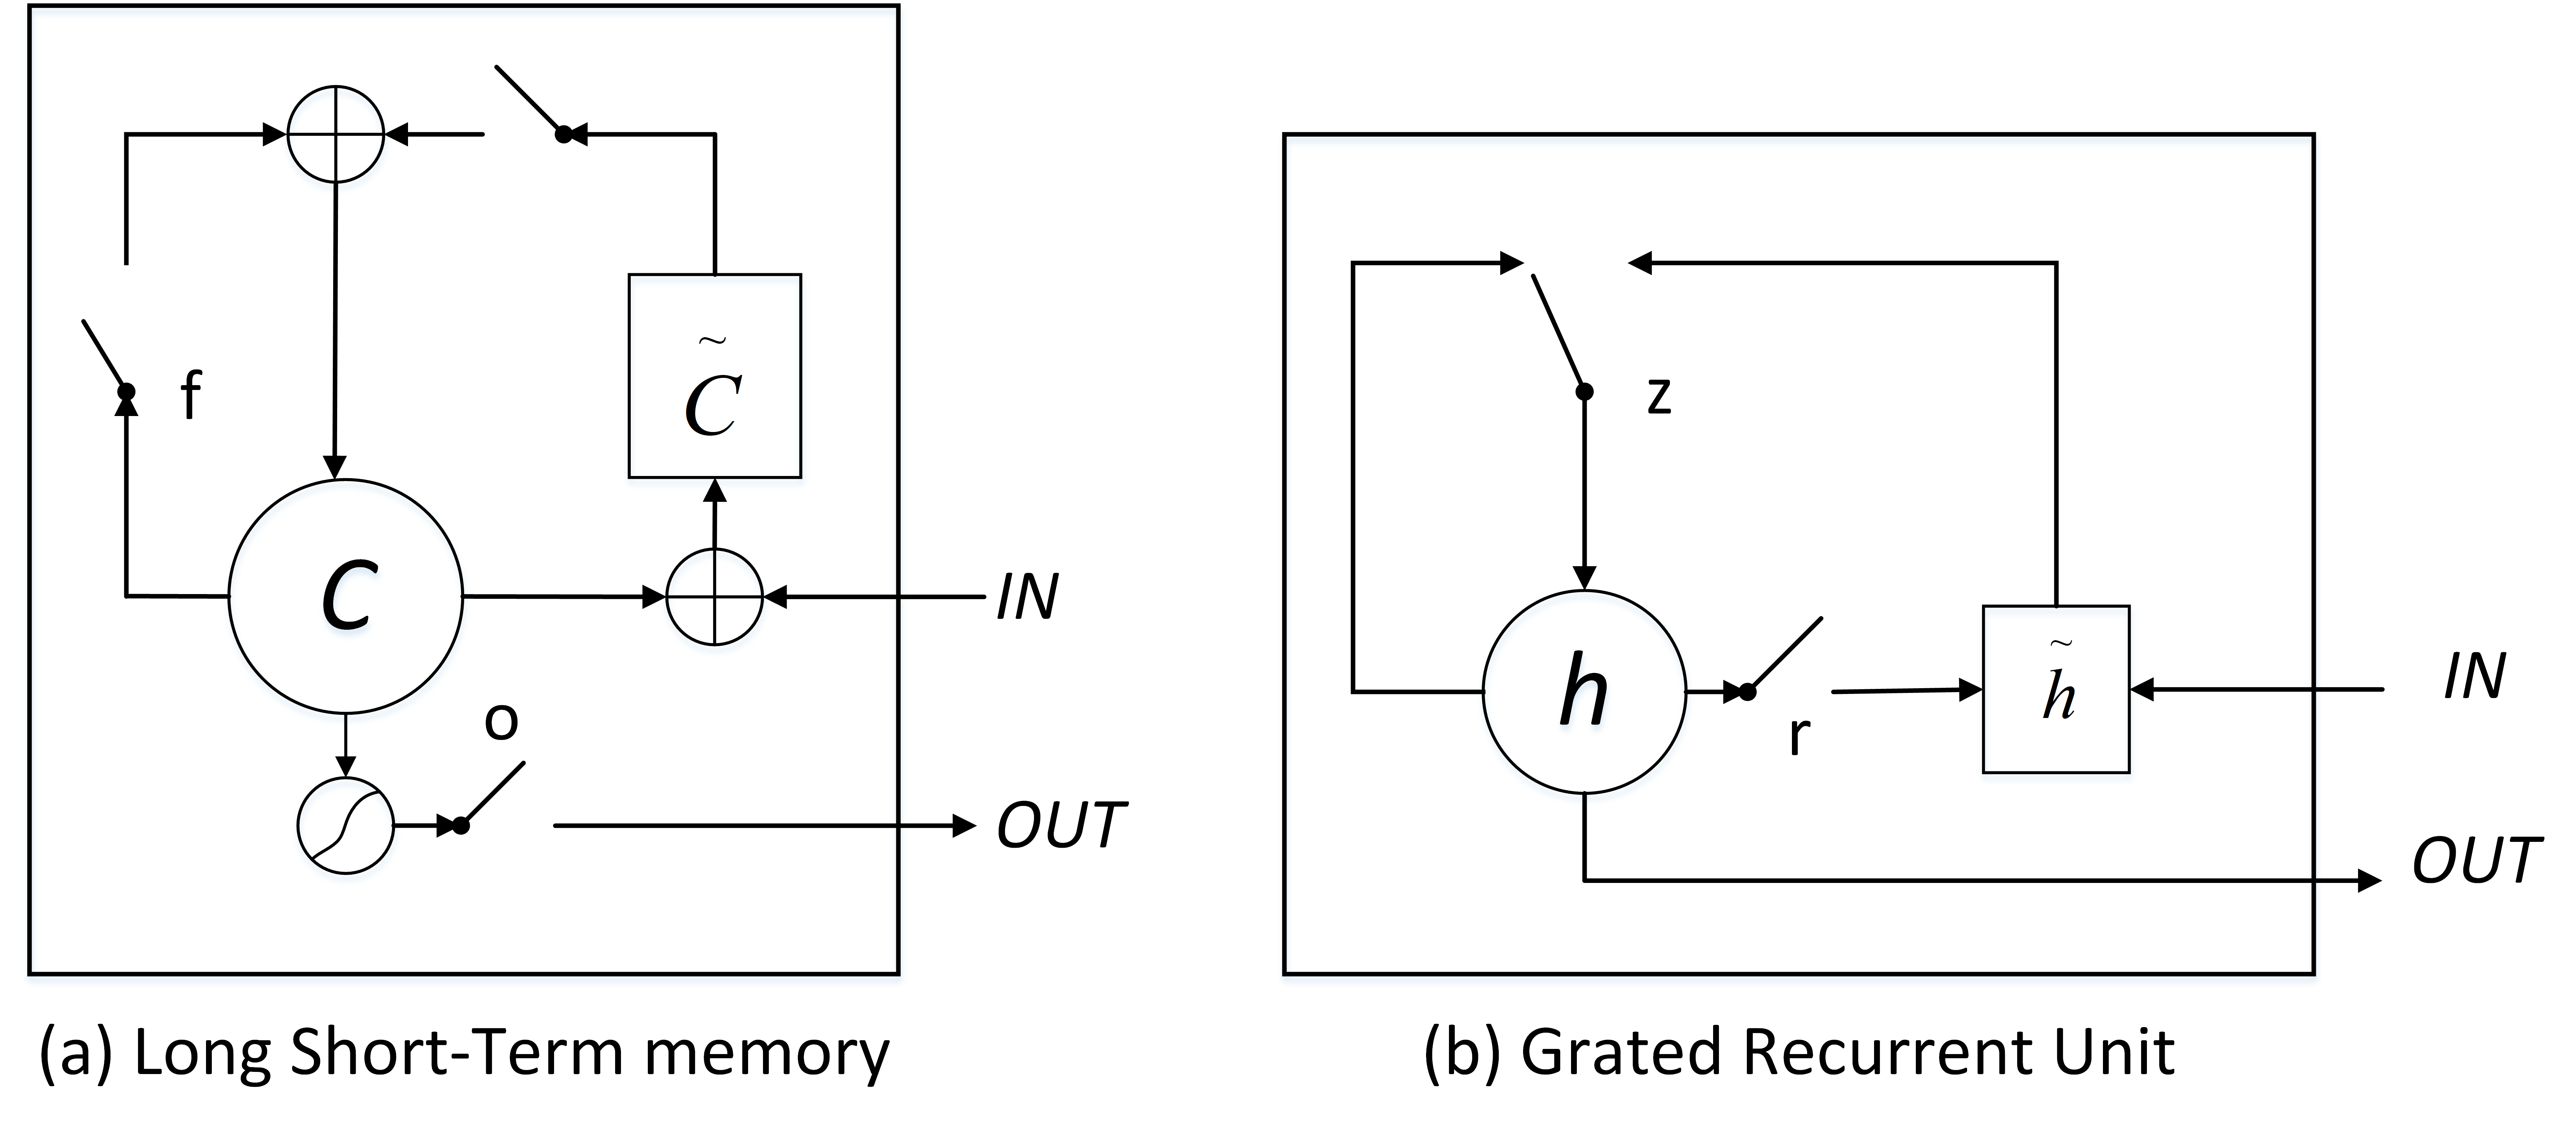
\includegraphics{./img/ch6/figure_6.6.6_2.png}
%\caption{}
%\end{figure}

从上图可以看出,二者结构十分相似,\textbf{不同在于}:

\begin{enumerate}
\def\labelenumi{\arabic{enumi}.}
% \tightlist
\item
  new memory都是根据之前state及input进行计算,但是GRUs中有一个reset
  gate控制之前state的进入量,而在LSTMs里没有类似gate;
\item
  产生新的state的方式不同,LSTMs有两个不同的gate,分别是forget gate (f
  gate)和input gate(i gate),而GRUs只有一种update gate(z gate);
\item
  LSTMs对新产生的state可以通过output gate(o
  gate)进行调节,而GRUs对输出无任何调节。
\end{enumerate}

\section{6.13
RNNs在NLP中典型应用?}\label{rnnsux5728nlpux4e2dux5178ux578bux5e94ux7528}

\textbf{(1)语言模型与文本生成(Language Modeling and Generating Text)}

​
给定一组单词序列,需要根据前面单词预测每个单词出现的可能性。语言模型能够评估某个语句正确的可能性,可能性越大,语句越正确。另一种应用便是使用生成模型预测下一个单词的出现概率,从而利用输出概率的采样生成新的文本。

\textbf{(2)机器翻译(Machine Translation)}

​
机器翻译是将一种源语言语句变成意思相同的另一种源语言语句,如将英语语句变成同样意思的中文语句。与语言模型关键的区别在于,需要将源语言语句序列输入后,才进行输出,即输出第一个单词时,便需要从完整的输入序列中进行获取。

\textbf{(3)语音识别(Speech Recognition)}

​
语音识别是指给定一段声波的声音信号,预测该声波对应的某种指定源语言语句以及计算该语句的概率值。

\textbf{(4)图像描述生成 (Generating Image Descriptions)}

​
同卷积神经网络一样,RNNs已经在对无标图像描述自动生成中得到应用。CNNs与RNNs结合也被应用于图像描述自动生成。
%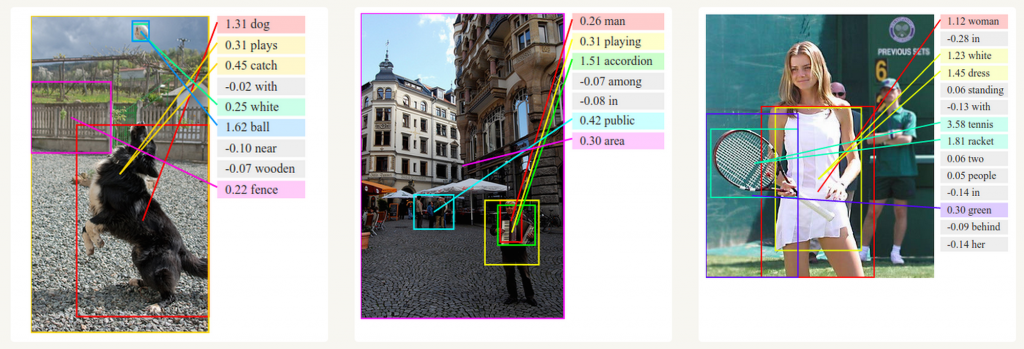
\includegraphics{./img/ch6/figure_6.4_1.png}

\section{6.13
常见的RNNs扩展和改进模型}\label{ux5e38ux89c1ux7684rnnsux6269ux5c55ux548cux6539ux8fdbux6a21ux578b}

\subsection{6.13.1 Simple RNNs(SRNs)}\label{simple-rnnssrns}

\begin{enumerate}
\def\labelenumi{\arabic{enumi}.}
% \tightlist
\item
  SRNs是一个三层网络,其在隐藏层增加了上下文单元。下图中的y是隐藏层,u是上下文单元。上下文单元节点与隐藏层中节点的连接是固定的,并且权值也是固定的。上下文节点与隐藏层节点一一对应,并且值是确定的。
\item
  在每一步中,使用标准的前向反馈进行传播,然后使用学习算法进行学习。上下文每一个节点保存其连接隐藏层节点上一步输出,即保存上文,并作用于当前步对应的隐藏层节点状态,即隐藏层的输入由输入层的输出与上一步的自身状态所决定。因此SRNs能够解决标准多层感知机(MLP)无法解决的对序列数据进行预测的问题。
  SRNs网络结构如下图所示:
\end{enumerate}

%\begin{figure}
%\centering
%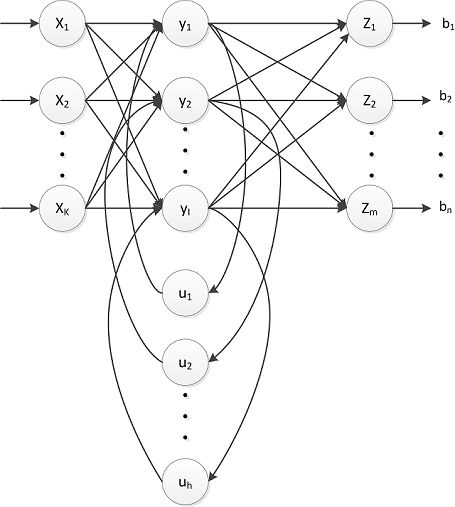
\includegraphics{./img/ch6/figure_6.6.1_1.png}
%\caption{}
%\end{figure}

\subsection{6.13.2 Bidirectional RNNs}\label{bidirectional-rnns}

​ Bidirectional
RNNs(双向网络)将两层RNNs叠加在一起,当前时刻输出(第t步的输出)不仅仅与之前序列有关,还与之后序列有关。例如:为了预测一个语句中的缺失词语,就需要该词汇的上下文信息。Bidirectional
RNNs是一个相对较简单的RNNs,是由两个RNNs上下叠加在一起组成的。输出由前向RNNs和后向RNNs共同决定。如下图所示:

%\begin{figure}
%\centering
%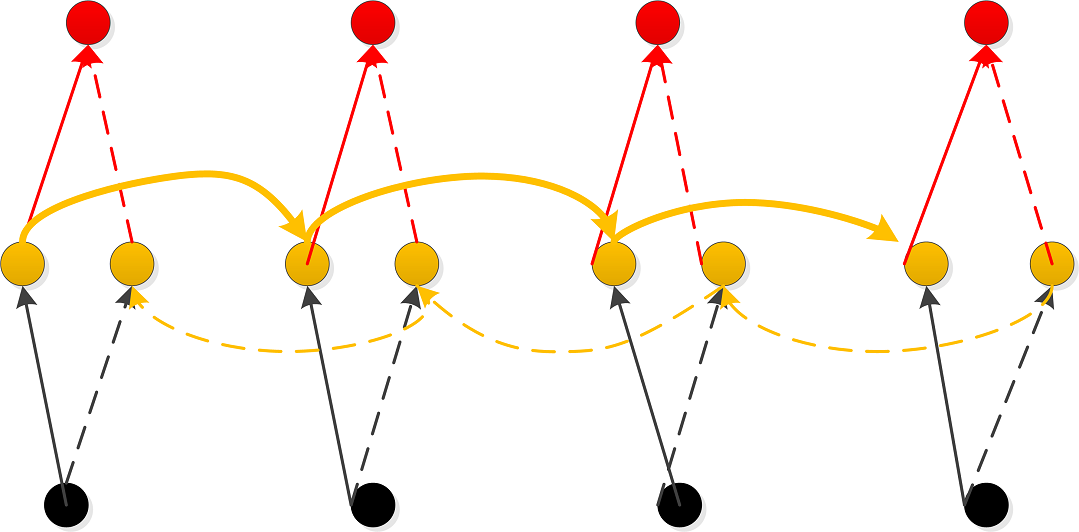
\includegraphics{./img/ch6/figure_6.6.2_1.png}
%\caption{}
%\end{figure}

\subsection{6.13.3 Deep RNNs}\label{deep-rnns}

​ Deep RNNs与Bidirectional
RNNs相似,其也是又多层RNNs叠加,因此每一步的输入有了多层网络。该网络具有更强大的表达与学习能力,但是复杂性也随之提高,同时需要更多的训练数据。Deep
RNNs的结构如下图所示: %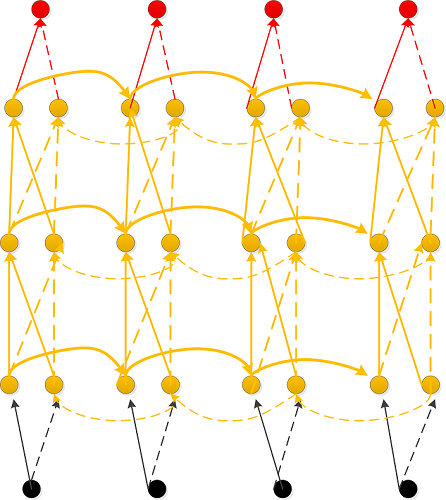
\includegraphics{./img/ch6/figure_6.6.3_1.png}

\subsection{6.13.4 Echo State
Networks(ESNs)}\label{echo-state-networksesns}

\textbf{ESNs特点}:

\begin{enumerate}
\def\labelenumi{\arabic{enumi}.}
% \tightlist
\item
  它的核心结构为一个随机生成、且保持不变的储备池(Reservoir)。储备池是大规模随机生成稀疏连接(SD通常保持1\%~5\%,SD表示储备池中互相连接的神经元占总神经元个数N的比例)的循环结构;
\item
  从储备池到输出层的权值矩阵是唯一需要调整的部分;
\item
  简单的线性回归便能够完成网络训练;
\end{enumerate}

\textbf{ESNs基本思想}:

​
使用大规模随机连接的循环网络取代经典神经网络中的中间层,从而简化网络的训练过程。
网络中的参数包括: (1)W - 储备池中节点间连接权值矩阵; (2)Win -
输入层到储备池之间连接权值矩阵,表明储备池中的神经元之间是相互连接;
(3)Wback -
输出层到储备池之间的反馈连接权值矩阵,表明储备池会有输出层来的反馈;
(4)Wout -
输入层、储备池、输出层到输出层的连接权值矩阵,表明输出层不仅与储备池连接,还与输入层和自己连接。
(5)Woutbias - 输出层的偏置项。

​ ESNs的结构如下图所示:

%\begin{figure}
%\centering
%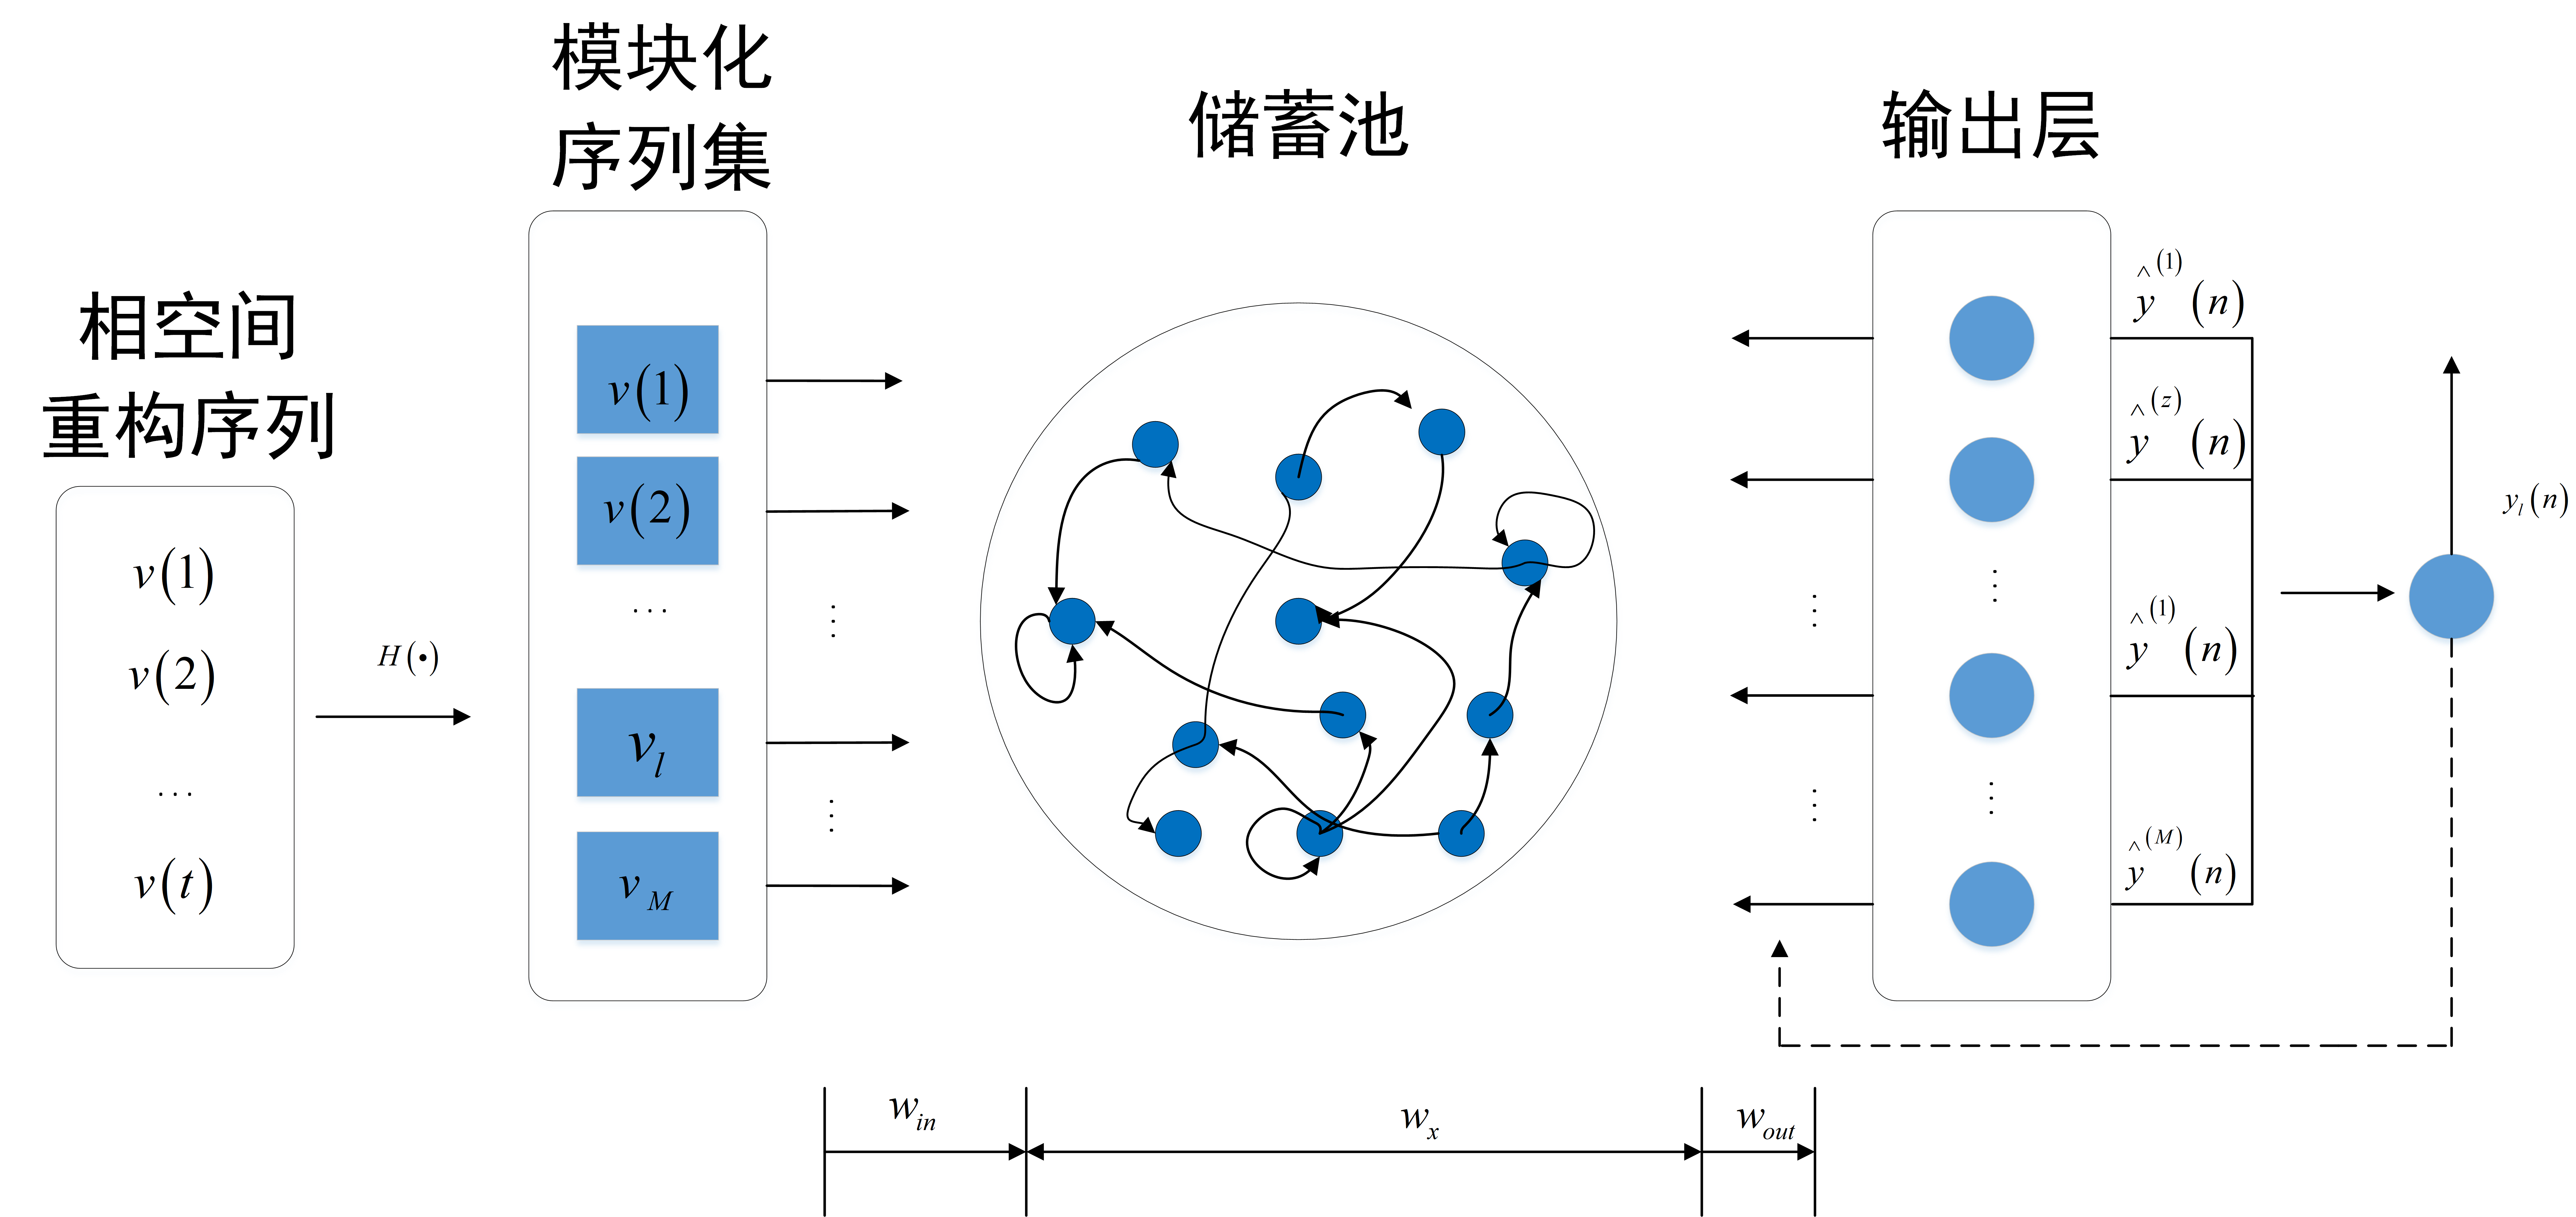
\includegraphics{./img/ch6/figure_6.6.4_2.png}
%\caption{}
%\end{figure}

\subsection{6.13.4 Gated Recurrent Unit Recurrent Neural
Networks}\label{gated-recurrent-unit-recurrent-neural-networks}

GRUs是一般的RNNs的变型版本,其主要是从以下两个方面进行改进。

\begin{enumerate}
\def\labelenumi{\arabic{enumi}.}
\item
  以语句为例,序列中不同单词处的数据对当前隐藏层状态的影响不同,越前面的影响越小,即每个之前状态对当前的影响进行了距离加权,距离越远,权值越小。
\item
  在产生误差error时,其可能是由之前某一个或者几个单词共同造成,所以应当对对应的单词weight进行更新。GRUs的结构如下图所示。GRUs首先根据当前输入单词向量word
  vector以及前一个隐藏层状态hidden state计算出update gate和reset
  gate。再根据reset gate、当前word vector以及前一个hidden
  state计算新的记忆单元内容(new memory content)。当reset
  gate为1的时候,new memory content忽略之前所有memory
  content,最终的memory是由之前的hidden state与new memory
  content一起决定。
\end{enumerate}

%\begin{figure}
%\centering
%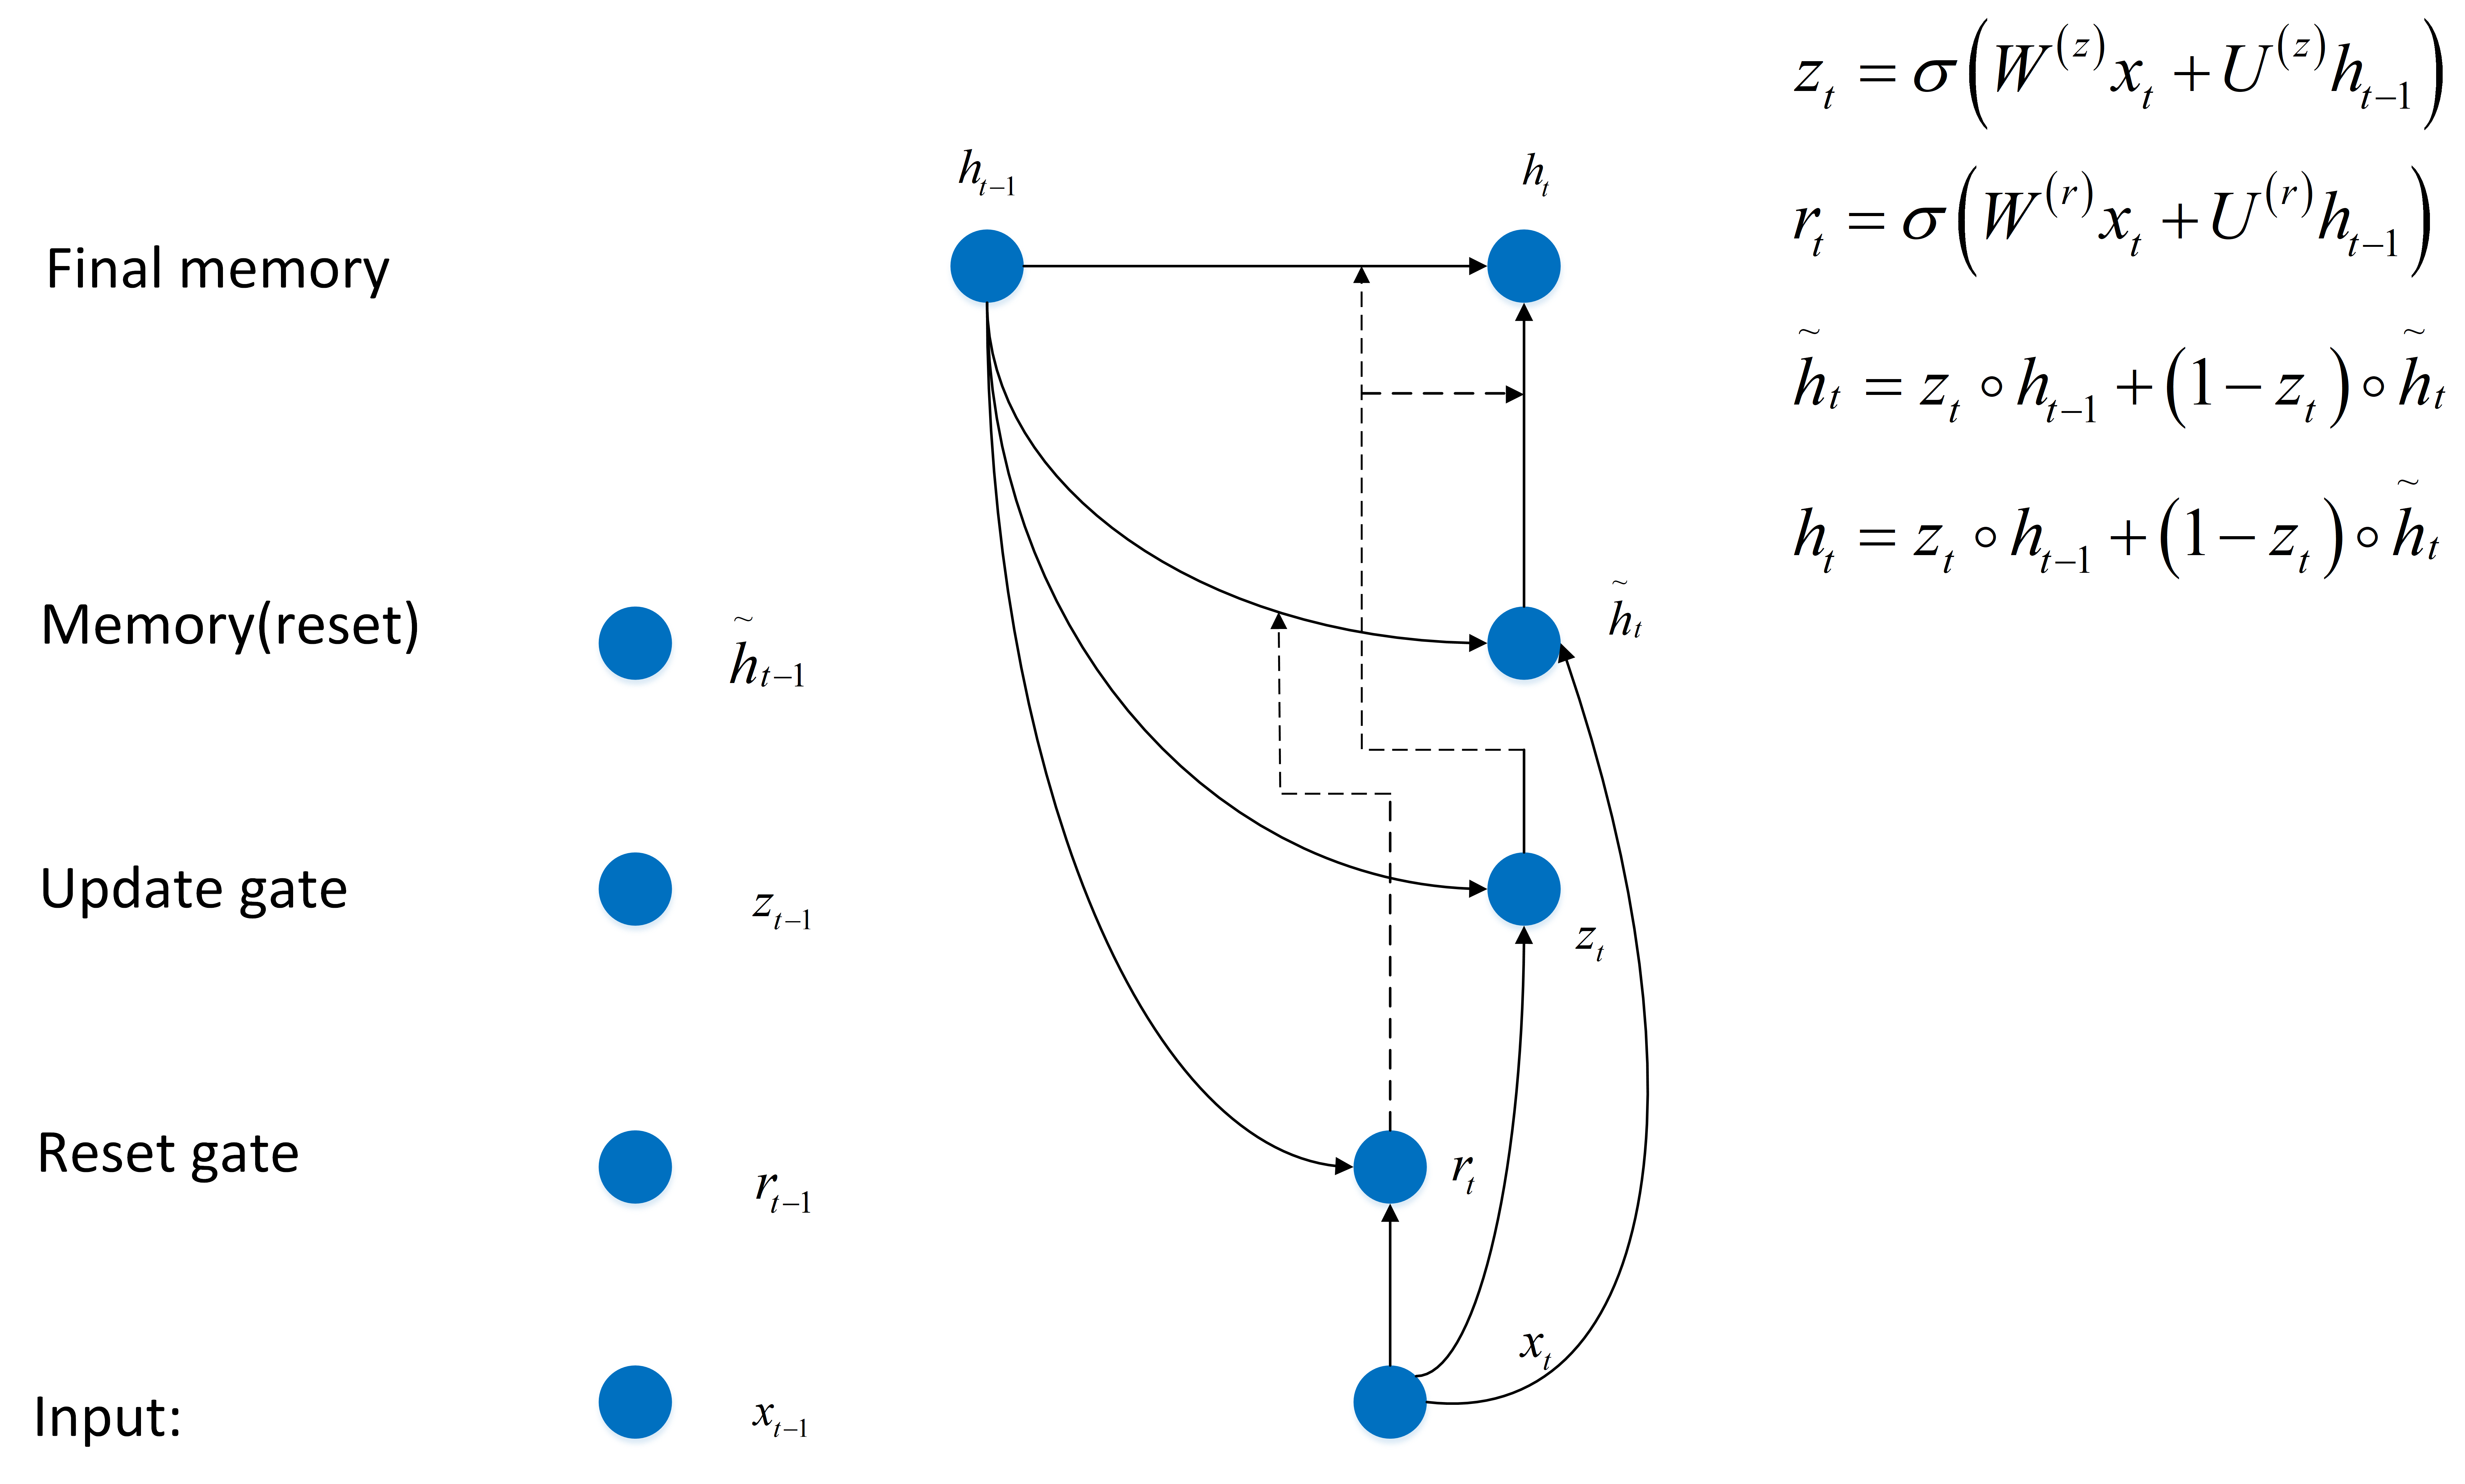
\includegraphics{./img/ch6/figure_6.6.5_1.png}
%\caption{}
%\end{figure}

\subsection{6.13.5 Bidirectional LSTMs}\label{bidirectional-lstms}

\begin{enumerate}
\def\labelenumi{\arabic{enumi}.}
% \tightlist
\item
  与bidirectional RNNs 类似,bidirectional
  LSTMs有两层LSTMs。一层处理过去的训练信息,另一层处理将来的训练信息。
\item
  在bidirectional
  LSTMs中,通过前向LSTMs获得前向隐藏状态,后向LSTMs获得后向隐藏状态,当前隐藏状态是前向隐藏状态与后向隐藏状态的组合。
\end{enumerate}

\subsection{6.13.6 Stacked LSTMs}\label{stacked-lstms}

\begin{enumerate}
\def\labelenumi{\arabic{enumi}.}
% \tightlist
\item
  与deep rnns 类似,stacked LSTMs
  通过将多层LSTMs叠加起来得到一个更加复杂的模型。
\item
  不同于bidirectional LSTMs,stacked LSTMs只利用之前步骤的训练信息。
\end{enumerate}

\subsection{6.13.7 Clockwork
RNNs(CW-RNNs)}\label{clockwork-rnnscw-rnns}

​
CW-RNNs是RNNs的改良版本,其使用时钟频率来驱动。它将隐藏层分为几个块(组,Group/Module),每一组按照自己规定的时钟频率对输入进行处理。为了降低RNNs的复杂度,CW-RNNs减少了参数数量,并且提高了网络性能,加速网络训练。CW-RNNs通过不同隐藏层模块在不同时钟频率下工作来解决长时依赖问题。将时钟时间进行离散化,不同的隐藏层组将在不同时刻进行工作。因此,所有的隐藏层组在每一步不会全部同时工作,这样便会加快网络的训练。并且,时钟周期小组的神经元不会连接到时钟周期大组的神经元,只允许周期大的神经元连接到周期小的(组与组之间的连接以及信息传递是有向的)。周期大的速度慢,周期小的速度快,因此是速度慢的神经元连速度快的神经元,反之则不成立。

​
CW-RNNs与SRNs网络结构类似,也包括输入层(Input)、隐藏层(Hidden)、输出层(Output),它们之间存在前向连接,输入层到隐藏层连接,隐藏层到输出层连接。但是与SRN不同的是,隐藏层中的神经元会被划分为若干个组,设为\(g​\),每一组中的神经元个数相同,设为\(k​\),并为每一个组分配一个时钟周期\(T_i\epsilon\{T_1,T_2,...,T_g\}​\),每一组中的所有神经元都是全连接,但是组\(j​\)到组\(i​\)的循环连接则需要满足\(T_j​\)大于\(T_i​\)。如下图所示,将这些组按照时钟周期递增从左到右进行排序,即\(T_1<T_2<...<T_g​\),那么连接便是从右到左。例如:隐藏层共有256个节点,分为四组,周期分别是{[}1,2,4,8{]},那么每个隐藏层组256/4=64个节点,第一组隐藏层与隐藏层的连接矩阵为64$\times​\(64的矩阵,第二层的矩阵则为64\)\times​\(128矩阵,第三组为64\)\times​\((3\)\times​\(64)=64\)\times​\(192矩阵,第四组为64\)\times​\((4\)\times​\(64)=64\)\times​$256矩阵。这就解释了上一段中速度慢的组连接到速度快的组,反之则不成立。

\textbf{CW-RNNs的网络结构如下图所示}:

%\begin{figure}
%\centering
%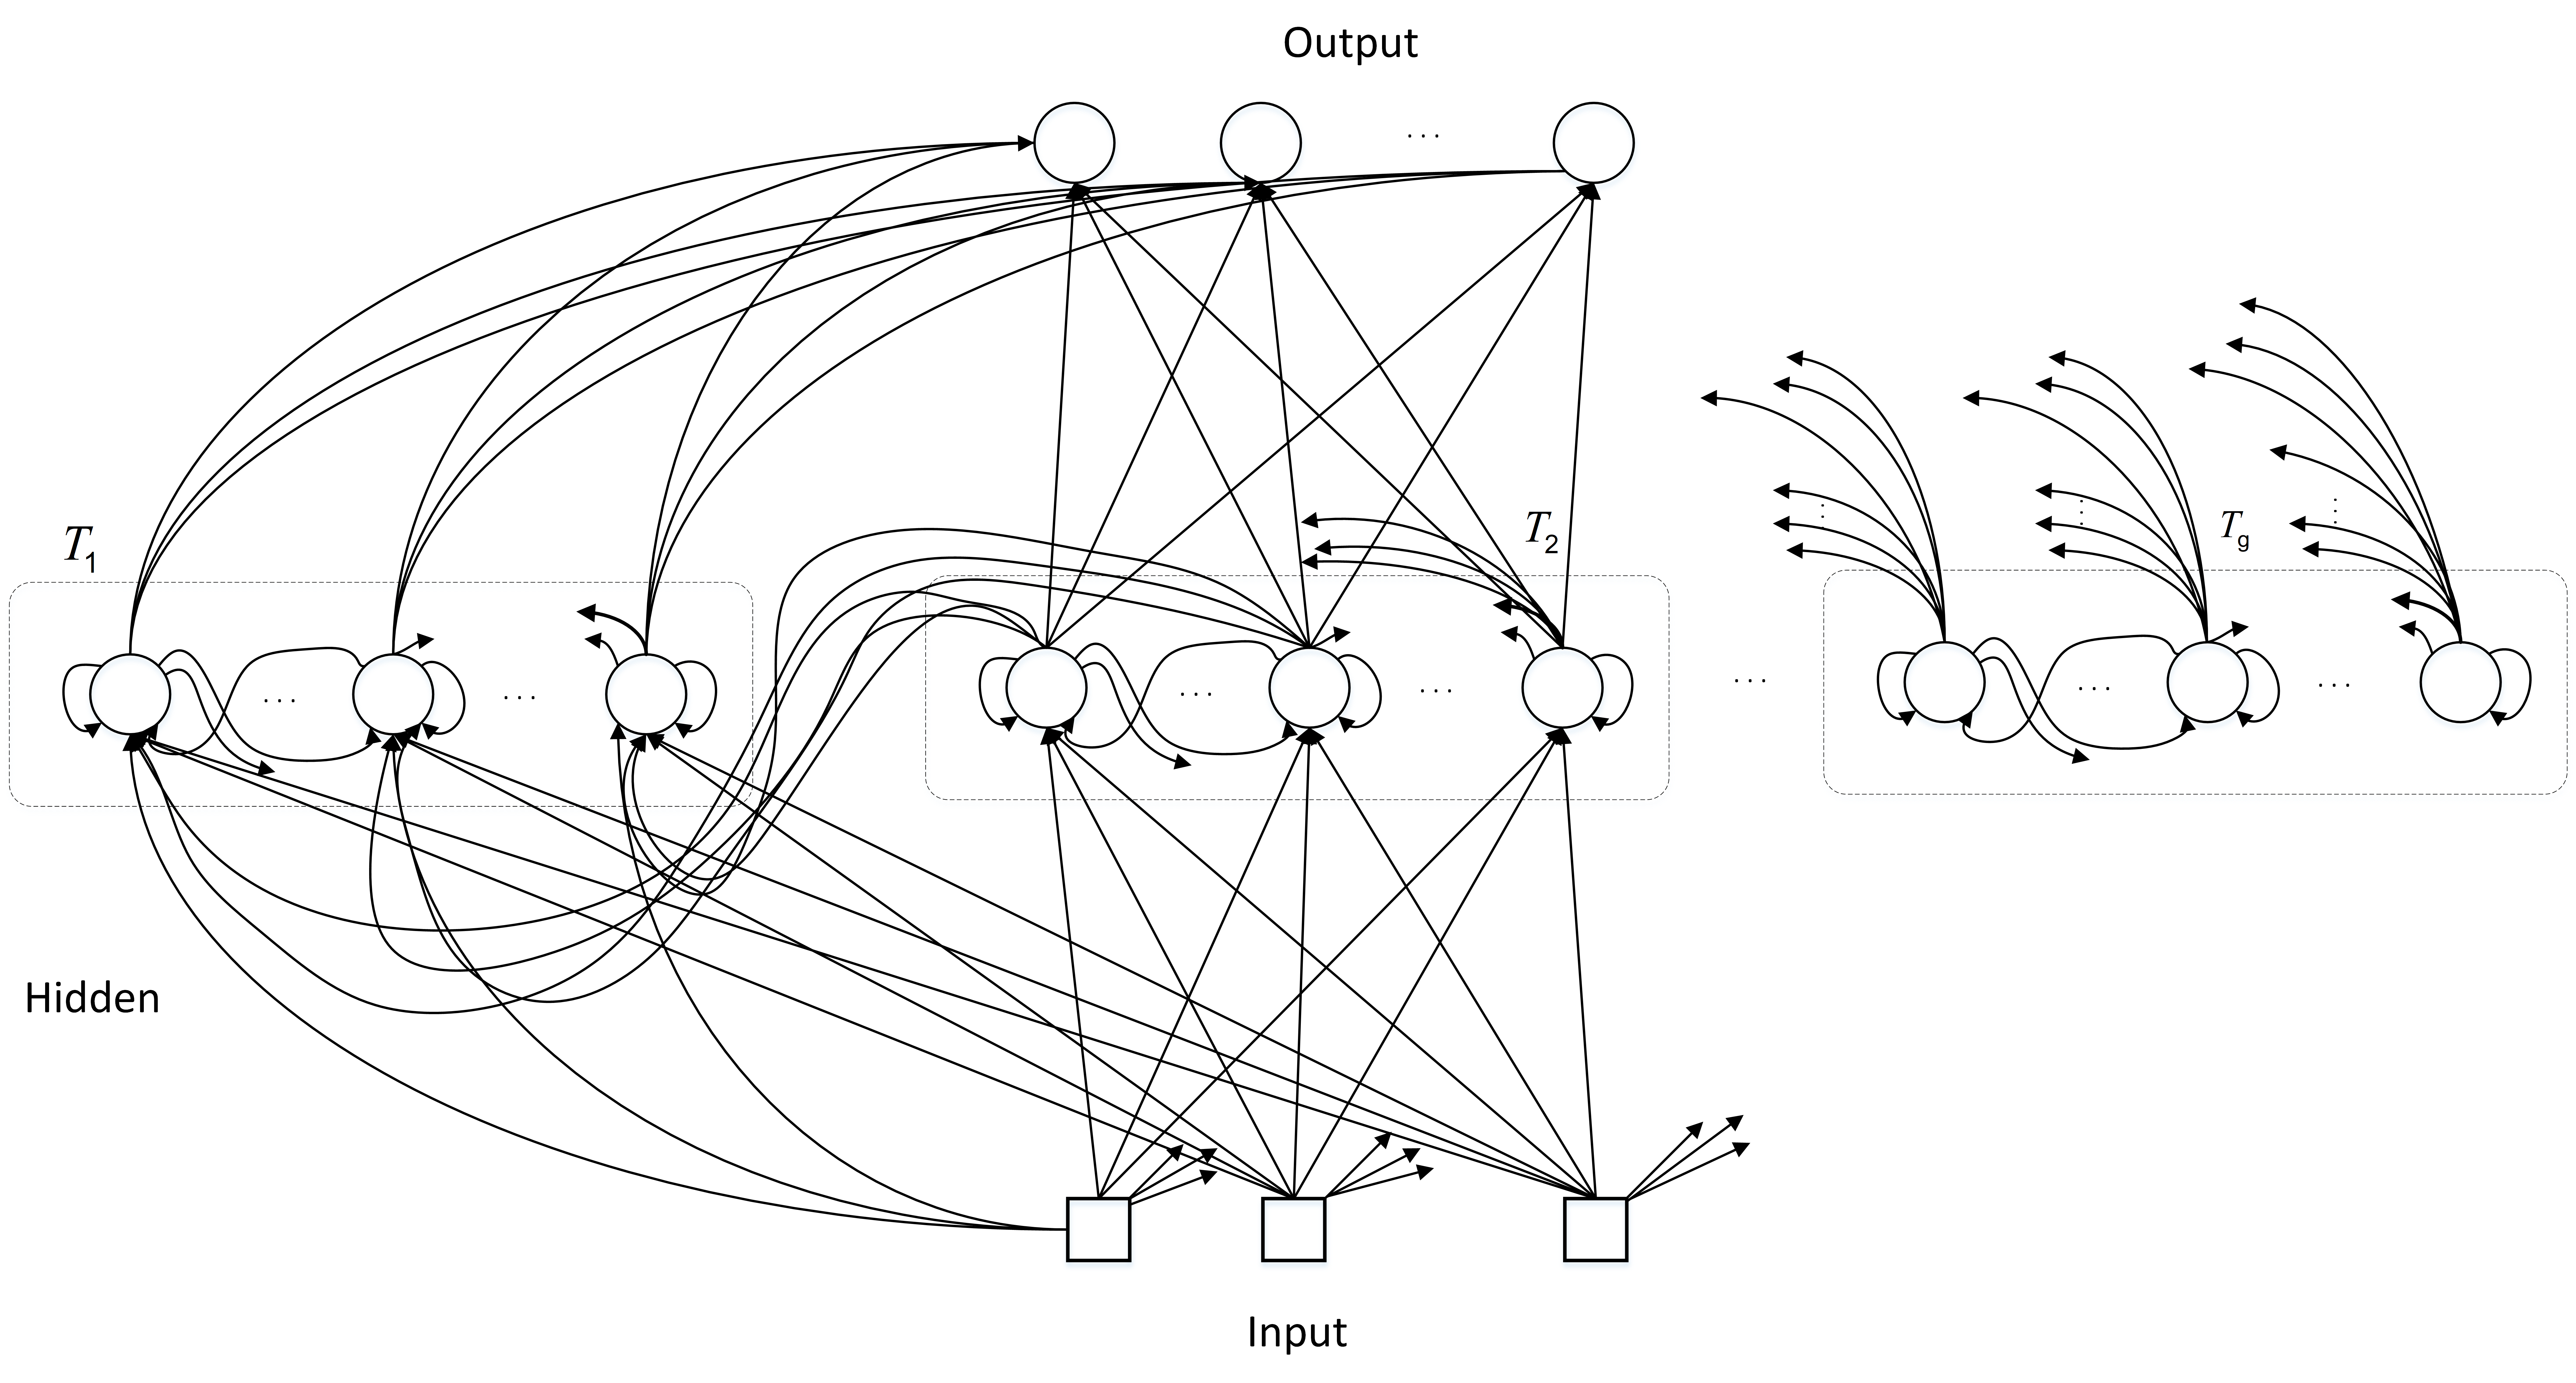
\includegraphics{./img/ch6/figure_6.6.7_1.png}
%\caption{}
%\end{figure}

\subsection{6.13.8 CNN-LSTMs}\label{cnn-lstms}

\begin{enumerate}
\def\labelenumi{\arabic{enumi}.}
% \tightlist
\item
  为了同时利用CNN以及LSTMs的优点,CNN-LSTMs被提出。在该模型中,CNN用于提取对象特征,LSTMs用于预测。CNN由于卷积特性,其能够快速而且准确地捕捉对象特征。LSTMs的优点在于能够捕捉数据间的长时依赖性。
\end{enumerate}

% \section{参考文献}\label{ux53c2ux8003ux6587ux732e}

% {[}1{]} 何之源.https://zhuanlan.zhihu.com/p/28054589.

% {[}2{]} http://colah.github.io/posts/2015-08-Understanding-LSTMs/

% {[}3{]} https://blog.csdn.net/zhaojc1995/article/details/80572098

% {[}4{]} Graves A. Supervised Sequence Labelling with Recurrent Neural
% Networks{[}J{]}. Studies in Computational Intelligence, 2008, 385.

% {[}5{]} Graves A. Generating Sequences With Recurrent Neural
% Networks{[}J{]}. Computer Science, 2013.

% {[}6{]} Greff K , Srivastava R K , Koutník, Jan, et al. LSTM: A Search
% Space Odyssey{[}J{]}. IEEE Transactions on Neural Networks \& Learning
% Systems, 2015, 28(10):2222-2232.

% {[}7{]} Lanchantin J, Singh R, Wang B, et al. DEEP MOTIF DASHBOARD:
% VISUALIZING AND UNDERSTANDING GENOMIC SEQUENCES USING DEEP NEURAL
% NETWORKS.{[}J{]}. Pacific Symposium on Biocomputing Pacific Symposium on
% Biocomputing, 2016, 22:254.

% {[}8{]} Pascanu R , Mikolov T , Bengio Y . On the difficulty of training
% Recurrent Neural Networks{[}J{]}. 2012.

% {[}9{]} Hochreiter S. The Vanishing Gradient Problem During Learning
% Recurrent Neural Nets and Problem Solutions{[}J{]}. International
% Journal of Uncertainty, Fuzziness and Knowledge-Based Systems, 1998,
% 06(02):-.

% {[}10{]} Dyer C, Kuncoro A, Ballesteros M, et al. Recurrent Neural
% Network Grammars{[}C{]}// Conference of the North American Chapter of
% the Association for Computational Linguistics: Human Language
% Technologies. 2016.

% {[}11{]} Mulder W D , Bethard S , Moens M F . A survey on the
% application of recurrent neural networks to statistical language
% modeling.{[}M{]}. Academic Press Ltd. 2015.

% {[}12{]} Graves A. Generating Sequences With Recurrent Neural
% Networks{[}J{]}. Computer Science, 2013.

% {[}13{]} Zhang B, Xiong D, Su J. Neural Machine Translation with Deep
% Attention{[}J{]}. IEEE Transactions on Pattern Analysis and Machine
% Intelligence, 2018, PP(99):1-1.

% {[}14{]} \url{https://github.com/xuanyuansen/scalaLSTM}

% {[}15{]} Deep Learning,Ian Goodfellow Yoshua Bengio and Aaron
% Courville,Book in preparation for MIT Press,2016;

% {[}16{]} http://colah.github.io/posts/2015-08-Understanding-LSTMs/

% {[}17{]} Greff K, Srivastava R K, Koutník J, et al. LSTM: A Search Space
% Odyssey{[}J{]}. IEEE Transactions on Neural Networks \& Learning
% Systems, 2016, 28(10):2222-2232.

% {[}18{]} Yao K , Cohn T , Vylomova K , et al. Depth-Gated Recurrent
% Neural Networks{[}J{]}. 2015.

% {[}19{]} Koutník J, Greff K, Gomez F, et al. A Clockwork RNN{[}J{]}.
% Computer Science, 2014:1863-1871.

% {[}20{]} Gers F A , Schmidhuber J . Recurrent nets that time and
% count{[}C{]}// Neural Networks, 2000. IJCNN 2000, Proceedings of the
% IEEE-INNS-ENNS International Joint Conference on. IEEE, 2000.

% {[}21{]} Li S, Wu C, Hai L, et al. FPGA Acceleration of Recurrent Neural
% Network Based Language Model{[}C{]}// IEEE International Symposium on
% Field-programmable Custom Computing Machines. 2015.

% {[}22{]} Mikolov T , Kombrink S , Burget L , et al. Extensions of
% recurrent neural network language model{[}C{]}// Acoustics, Speech and
% Signal Processing (ICASSP), 2011 IEEE International Conference on. IEEE,
% 2011.

% {[}23{]} Graves A . Generating Sequences With Recurrent Neural
% Networks{[}J{]}. Computer Science, 2013.

% {[}24{]} Sutskever I , Vinyals O , Le Q V . Sequence to Sequence
% Learning with Neural Networks{[}J{]}. 2014.

% {[}25{]} Liu B, Lane I. Joint Online Spoken Language Understanding and
% Language Modeling with Recurrent Neural Networks{[}J{]}. 2016.

% {[}26{]} Graves A, Mohamed A R, Hinton G. Speech recognition with deep
% recurrent neural networks{[}C{]}// IEEE International Conference on
% Acoustics. 2013.

% {[}27{]} https://cs.stanford.edu/people/karpathy/deepimagesent/

% {[}28{]} Cho K, Van Merriënboer B, Gulcehre C, et al. Learning phrase
% representations using RNN encoder-decoder for statistical machine
% translation{[}J{]}. arXiv preprint arXiv:1406.1078, 2014.
